\documentclass[a4paper]{report}

\usepackage[utf8]{inputenc}
\usepackage[T1]{fontenc}
\usepackage[francais]{babel}
\usepackage{graphicx}

\title{Projet Station Météo\\Compte Rendu Équipe 5}
\author{Kévin \bsc{Vythelingum} \cr Lamine \bsc{Saidoun} \cr Hugo \bsc{Vérité} \cr Yannick \bsc{Larvor} \cr Yannick \bsc{Riou} \cr Adrien \bsc{Coudray} \cr Jean-Michel \bsc{Nokaya} \cr Fabien \bsc{Jaraczewski}}
\date{\today}

\makeatletter\@addtoreset{section}{part}\makeatother
\renewcommand{\thepart}{\arabic{part}}
\renewcommand{\thesection}{\thepart.\arabic{section}}

\renewcommand{\thefigure}{\arabic{figure}}

\begin{document}

\maketitle
\tableofcontents

\chapter*{Introduction}
La météo Lannionaise est particulière, c'est pourquoi il peut être intéressant de relever quelques informations pour son étude.
Parmi celles-ci, certaines sont indispensables comme la température, la vitesse du vent et la pluviométrie.
Dans cette perspective, nous développeront une station météo disposant d'un écran LCD qui affichera les informations demandées par l'utilisateur, complété de signaux sonores.
L'ensemble sera piloté à partir d'une télécommande.
L'objectif de ce projet est de mettre en oeuvre les différents périphériques mis à disposition au sein d'une équipe.

Plus précisément le cahier des charges qui nous était fournit avait pour objet de :
\begin{itemize}
\item Désigner un chef de projet
\item Mesurer la vitesse du vent
\item Mesurer la pluviométrie
\item Mesurer la température
\item Réceptionner le signal d'une télécommande
\item Gérer un afficheur LCD
\item Programmer une RTC
\item Générer une note
\end{itemize}

Concernant ce compte-rendu, il est découpé en huit parties, chacune correspondant à un poste occupé par un membre de l'équipe.
Chaque membre aura donc pris soin d'expliquer sa contribution au projet en illustrant ses propos d'une part par son code, d'autre part grâce à des images tirés de la documentation.
Aussi, la conclusion comportera un état d'avancement de la station.
En ce qui concerne le code en lui-même, il ne fera pas parti du rapport mais pourra se trouver en annexe.

\part{Chef de projet\\-\\Kévin \bsc{Vythelingum}}
\section{Cahier des charges}
Cette partie du projet consiste d'abord à répartir les tâches et le matériel entre les membres de l'équipe.
En effet, il ne faut pas que deux personnes se servent du même Timer pour deux choses différentes par exemple.
Ensuite, il faut mettre en place un Timer pour la base de temps générale afin de synchroniser les mises à jour des données météo.
Enfin, la préparation du programme principal permettra d'assembler les différents codes de l'équipe.

\section{Répartition des tâches et du matériel}
Dans l'objectif de prévenir les conflits qu'il pourrait y avoir au sein du projet, il a fallu définir une convention d'écriture pour les fonctions, les variables globales nécessaires ainsi l'attribution des différents composants de la carte.
J'ai réparti le matériel entre les membres de l'équipe de la manière suivante :

\subsection{Chef de projet}
Kévin \bsc{Vythelingum}
\paragraph{Hardware}
\begin{itemize}
\item Timer 0
\end{itemize}
\paragraph{Fonctions principales}
\begin{itemize}
\item \emph{main} : programme principal
\end{itemize}

\subsection{Anémomètre}
Lamine \bsc{Saidoun}
\paragraph{Hardware}
\begin{itemize}
\item Timer 1
\item PIOB (broche PB23)
\end{itemize}
\paragraph{Préfixe des fonctions}
\begin{itemize}
\item Les fonctions seront préfixées par \emph{VENT\_}
\end{itemize}
\paragraph{Variables globales}
\begin{itemize}
\item \emph{vitesseVent} : entier qui contient la vitesse du vent en km/h
\end{itemize}
\paragraph{Fonctions principales}
\begin{itemize}
\item \emph{VENT\_getVitesseVent} : retourne la vitesse du vent en km/h
\item \emph{VENT\_setVitesseVent} : met à jour \emph{vitesseVent}
\end{itemize}

\subsection{Datation}
Hugo \bsc{Vérité}
\paragraph{Hardware}
\begin{itemize}
\item RTC (Real Time Clock)
\end{itemize}
\paragraph{Préfixe des fonctions}
\begin{itemize}
\item Les fonctions seront préfixées par \emph{RTC\_}
\end{itemize}
\paragraph{Variables globales}
\begin{itemize}
\item \emph{realTime} : chaîne de caractères qui contient l’heure instantanée
\end{itemize}
\paragraph{Fonctions principales}
\begin{itemize}
\item \emph{RTC\_getRealTime} : retourne l’heure
\item \emph{RTC\_setRealTime} : met à jour \emph{realTime}
\end{itemize}

\subsection{Pluviométrie}
Yannick \bsc{Larvor}
\paragraph{Hardware}
\begin{itemize}
\item Timer 2
\item PIOB (broche PB3)
\end{itemize}
\paragraph{Préfixe des fonctions}
\begin{itemize}
\item Les fonctions seront préfixées par \emph{PLUV\_}
\end{itemize}
\paragraph{Variables globales}
\begin{itemize}
\item \emph{pluviometrie} : entier qui contient la pluviometrie depuis la dernière remise à zéro du pluviomètre
\item \emph{pluvHeureClear} : chaîne de caractères qui contient l’heure de dernière mise à zéro du pluviomètre
\end{itemize}
\paragraph{Fonctions principales}
\begin{itemize}
\item \emph{PLUV\_getPluviometrie} : retourne la pluviometrie en mm
\item \emph{PLUV\_setPluviometrie} : met à jour \emph{pluviometrie}
\item \emph{PLUV\_clearPluviometrie} : remet à zéro \emph{pluviometrie} et met à jour \emph{pluvHeureClear}
\item \emph{PLUV\_getHeureClear} : retourne l’heure \emph{pluvHeureClear}
\end{itemize}
\paragraph{Commentaire.}
Le choix de la mesure de la pluviométrie nécessite un commentaire. En effet, il est un peu particulier.
Nous avons opté pour le modèle d'un pluviomètre de jardin, c'est-à-dire qu'il se rempli tant que l'utilisateur ne l'aura pas "vidé" et affiche le résultat en mm.

\subsection{Température}
Yannick \bsc{Riou}
\paragraph{Hardware}
\begin{itemize}
\item CAN
\item carte d’extension
\end{itemize}
\paragraph{Préfixe des fonctions}
\begin{itemize}
\item Les fonctions seront préfixées par \emph{TEMP\_}
\end{itemize}
\paragraph{Variables globales}
\begin{itemize}
\item \emph{temperature} : entier qui contient la température en degrés celsius
\end{itemize}
\paragraph{Fonctions principales}
\begin{itemize}
\item \emph{TEMP\_getTemperature} : retourne la temperature en degrés celsius
\item \emph{TEMP\_setTemperature} : met à jour \emph{temperature}
\end{itemize}

\subsection{Télécommande}
Adrien \bsc{Coudray}
\paragraph{Hardware}
\begin{itemize}
\item Timer 3
\end{itemize}
\paragraph{Préfixe des fonctions}
\begin{itemize}
\item Les fonctions seront préfixées par \emph{RC\_}
\end{itemize}
\paragraph{Variables globales}
\begin{itemize}
\item \emph{select} : entier qui contient la dernière demande de l'utilisateur
\end{itemize}
\paragraph{Fonctions principales}
\begin{itemize}
\item \emph{RC\_getSelect} : retourne la sélection de l’utilisateur
\item \emph{RC\_setSelect} : met à jour \emph{select}
\end{itemize}

\subsection{Afficheur LCD}
Jean-Michel \bsc{Nokaya}
\paragraph{Hardware}
\begin{itemize}
\item USART 0
\end{itemize}
\paragraph{Préfixe des fonctions}
\begin{itemize}
\item Les fonctions seront préfixées par \emph{LCD\_}
\end{itemize}
\paragraph{Variables globales}
\begin{itemize}
\item pas de variable globale
\end{itemize}
\paragraph{Fonctions principales}
\begin{itemize}
\item \emph{LCD\_afficherTemp} : affiche la température à l’écran
\item \emph{LCD\_afficherVent} : affiche la vitesse du vent à l’écran
\item \emph{LCD\_afficherPluv} : affiche la pluviometrie à l’écran
\item \emph{LCD\_afficherPluvClear} : affiche un message du type "Le pluviomètre a été remis à 0"
\item \emph{LCD\_afficherHeure} : affiche l’heure à l’écran
\end{itemize}
\paragraph{Commentaire.}
Dans la version finale du projet, ces cinq fonctionnalités d'affichage sont remplies par une unique fonction \emph{LCD\_afficher(select)} qui prend en paramètre d'entrée le choix de l'utilisateur.

\subsection{Son}
Fabien \bsc{Jaraczewski}
\paragraph{Hardware}
\begin{itemize}
\item Timer 4
\end{itemize}
\paragraph{Préfixe des fonctions}
\begin{itemize}
\item Les fonctions seront préfixées par \emph{SON\_}
\end{itemize}
\paragraph{Variables globales}
\begin{itemize}
\item \emph{flagBip}
\end{itemize}
\paragraph{Fonctions principales}
\begin{itemize}
\item \emph{SON\_jouerAlarme} : génère une salve de bips
\item \emph{SON\_jouerBipOk} : génère un bip
\item \emph{SON\_jouerBipKo} : génère deux bips
\end{itemize}


\section{Fonctionnement du programme principal}
\subsection{Fonctionnement théorique}
Le programme principal utilise le Timer 0 pour générer des interruptions toutes les secondes. Ceci fourni une base de temps générale.
On utilise un compteur qui s'incrémente à chaque interruption pour diviser cette base de temps.
Cela nous permet de mettre à jour la vitesse du vent toutes les 3 secondes (on prend au maximum 2 s pour calculer la vitesse du vent) ainsi que la température toutes les 10 secondes (phénomène plus lent).
Aussi, on raffraichit l'afficheur LCD toutes les secondes pour tenir compte de l'heure et maintenir l'information affichée à jour.
La pluviométrie se met à jour avec sa propre interruption.
De même, le son est lancé par la télécommande lorqu'on appuie sur une touche et par les périphériques d'acquisition pour déclencher l'alarme lorsque certains seuils sont atteints.

\subsection{Fonctionnement en pratique}
En pratique, le programme principal ne fonctionne pas dans l'état actuel de cette manière.
En effet, au vu des difficultés à faire fonctionner la télécommande, j'ai ajouté au fonctionnement décrit précédemment une incrémentation de la variable globale \emph{select} toutes les 5 secondes.
Cela simule l'intervention d'un utilisateur qui choisirait tour à tour d'afficher les différentes informations disponibles.
De cette façon, la station météo répond tout de même à l'objectif de fournir des informations météorologiques en temps réel.

De plus, la station joue une musique d'accueil à sa mise sous tension grâce notamment au développement de la partie son par Fabien.

\section{Difficultés rencontrées}
En tant que chef de projet, mon rôle était d'avoir en permanence une vue d'ensemble des différentes parties.
Au-delà de ce rôle de coordinateur, j'ai aidé à résoudre certains problèmes qui bloquaient l'état d'avancement du projet.
C'est pourquoi je me suis finalement intéressé au détail d'une multitude de parties.
Parmi celles-ci, certaines ont particulièrement mis du temps à être résolues :
\subsection{Programmation de l'USART}
Cette partie s'est effectuée conjointement avec Jean-Michel.
Il était au début difficile de comprendre le fonctionnement de l'USART.
Or, cette partie était cruciale pour les autres membres de l'équipe afin qu'ils puissent tester leur programme sur la carte.
Comme c'était le premier composant sur lequel j'ai dû travaillé, il a fallu un peu de temps d'assimilation de la documentation technique.
Cette partie m'a aidé à appréhender les autres parties de la documentation et m'a donc été d'une grande aide pour la suite du projet.
Une fois que l'USART a fonctionné (affichage correct sur "Putty"), j'ai aidé Fabien dans la génération d'un son.
\subsection{Génération d'un son}
Je me suis impliqué dans la première partie de la tâche qui consistait à générer une note de musique.
Tout d'abord, Fabien avait choisi de générer le son à partir du signal créneau d'un timer.
Cependant, même en ayant une simulation correcte, aucun son ne sortait de la carte.
Il s'est avéré que les soudures avaient été effectuées en se fiant à des indications au niveau de l'interface avec la carte.
Or, ces indications étaient symétriquement opposées aux broches réelles. J'ai donc soudé à nouveau les différents composants de la carte et placé les cavaliers à la bonne place en m'aidant de la documentation plutôt que des marqueurs de la carte.
Ainsi, nous avons pu tester le son qui a été le premier élément à être validé à 100\% sur la carte.
Ce problème de soudure nous a évité de commettre à nouveau la même erreur pour le bouton poussoir du pluviomètre par exemple.

\part{La vitesse du vent\\-\\Lamine \bsc{Saidoun}}
\section{Cahier des charges}
Cette partie du projet consiste à réaliser un anémomètre pour mesurer la vitesse du vent.
Le but étant de calculer la vitesse du vent en km/h et de l'afficher sur l'écran LCD, pour cela il faut calculer la fréquence d'un signal rectangulaire délivré pas un ILS.
Cette fréquence est proportionnelle à la vitesse du vent (1Hz correspond à 1m/s) qu'il faudra convertir en km/h.

\begin{center}
	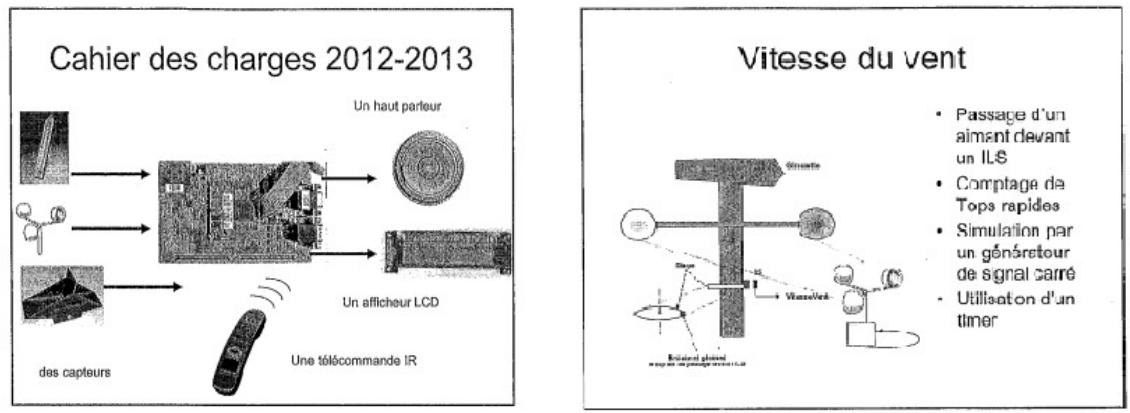
\includegraphics[scale=0.3]{images/VENT_fig1.png}
\end{center}

\section{Analyse}
\subsection{Périphériques}
Afin de concevoir l’anémomètre, j'utilise deux périphériques du $\mu$Controleur ARM : le timer 1 et la broche PB23 en entrée du port PIOB.

\begin{center}
	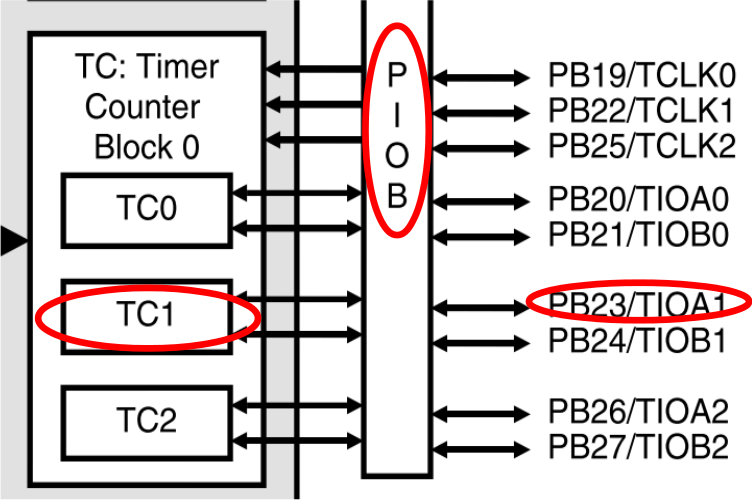
\includegraphics[scale=0.3]{images/VENT_fig2.png}
\end{center}

\subsection{Méthodologie}
Le principe étant de calculer la fréquence d'un signal rectangulaire x(t), deux méthodes sont possibles pour réaliser cela. La première consiste à comptabiliser le nombre de fronts montant de ce signal pendant une certaine durée T.
Cette méthode ne s'avère pas très efficace car le signal x(t) est de basse fréquence, il serait alors plus approprié de calculer la durée d'une période du signal en l'échantillonnant à une fréquence Fe (voir figure A) en utilisant un compteur (Timer) qu'on lance au premier front montant dont on récupère ensuite la valeur au prochain front montant.

\begin{center}
	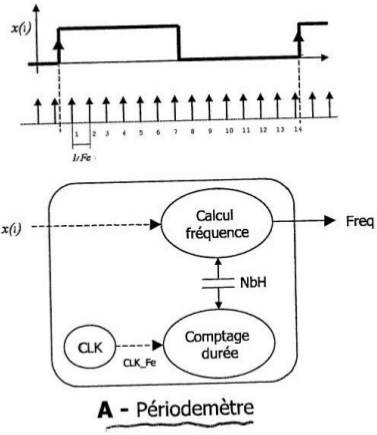
\includegraphics[scale=0.4]{images/VENT_fig3.png}
\end{center}

\subsection{Mode de fonctionnement}
Le Timer 1 sera utilisé en mode Capture et sera sensible aux fronts montants du signal sur la broche PB23.
On choisira une horloge de base MCK1024 pour obtenir une période d'échantillonnage de 32$\mu$s.

On notera qu'il peut y avoir deux situation possibles :

Lancement du Timer 1
\begin{itemize}
\item Premier cas : Présence de vent suffisant pour la mesure
	\begin{itemize}
		\item Chargement de la valeur du compteur dans RA sur front montant de x(t).
		\item Génération d'une interruption sur le même front d'horloge.
			\begin{itemize}
				\item Mise à jour d'un flag
				\item Récupération de la valeur du registre RA dans une variable intermédiaire
			\end{itemize}
		\item Calcul de la vitesse et mise à jour de la variable globale \texttt{vitesseVent}.
	\end{itemize}
\item Deuxième cas : Absence de vent (pas de fronts)
	\begin{itemize}
		\item Débordement du Timer 1.
		\item \texttt{vitesseVent = 0}.
	\end{itemize}
\end{itemize}

\section{Réalisation}
La réalisation de l'application Anémomètre s'est faite en plusieurs partie.
\subsection{Configuration des périphériques}
Afin de réaliser la fonction souhaitée, il a fallu configurer certains périphériques du microcontrôleur à l'aide de routines d'initialisation. Ces périphériques sont :
\begin{itemize}
\item Le PIOB : pour la configuration de la broche PB23 en entrée.
\item Le timer1 : configuration du registre de contrôle \texttt{TC1\_CMR}
	(Choix de l'entrée TIOA(PB23) ; sensibilisation sur front montant de TIOA ; permission d'interruptions ...etc).
\item L'AIC : Mise au point de la routine d'interruption
\end{itemize}

\subsection{Codage des procédures}
Les différentes procédures tiennent compte des contraintes matérielles (périphériques...) et leurs prototypes sont :
\begin{verbatim}
/* Initialisation des paramètre de l'application vent (utilisable par le main) */
void VENT_initialisation(void);
/* Procédure qui calcul la vitesse du vent en km/h */
void Vent_calcul_vitesseVent(void);
/* Procédure permettant la mise à jour de la vitesse du vent (utilisable par le main)*/
void VENT_setVitesseVent(void);
/* Procédure interne d'initialisation du timer1*/
void VENT_init_timerTC1(void);
/* Procédure interne d'initialisation de l'AIC */
void VENT_init_AIC(void);
/* Procédure interne d'initialisation du PIOA */
void VENT_init_PIOB(void);
/* Procédure d'interruption Timer */
__irq void VENT_interupt_timer(void);
/* Procédure de démarrage du compteur */
void Vent_Start_timer(void);
\end{verbatim}

\subsection{Configuration matérielle}
Afin de pouvoir injecter le signal venant de l'ILS sur la broche PB23 du $\mu$C, il fallait d'abord effectuer un câblage particulier sur la carte d’extension, ensuite poser des cavaliers dans la bonne position pour un bon aiguillage.

\section{Conclusion}
L'application Anémomètre réalisée fonctionne parfaitement en respectant le cahier des charges, la vitesse est représentée en km/h sur l'afficheur LCD lors de l’exécution du programme principal.
La réalisation de cette partie m'a permis non seulement de bien manipuler certains périphériques du microcontrôleur, mais aussi de savoir résoudre des problèmes de code et surmonter les contraintes matérielles.


\part{La datation\\-\\Hugo \bsc{Vérité}}
\section{Introduction}
L'objectif de ce TP est de réaliser une station météo à l'aide d'une carte ARM ainsi que de plusieurs périphériques.
Cette station doit être capable d'effectuer diverses taches comme par exemple indiquer la température ou la pluviométrie.
La tâche qui m'a été attribuée est de créer des fonctions capables de renvoyer l'heure et la date indiquées par la RTC (Real Time Clock) de l'ARM.

\section{Travail personnel}
J'ai, dans un premier temps effectué les différentes fonctions permettant de lire et retourner l'heure et la date contenue dans les registres TIMR et CALR.
J'ai donc d'abord créé les fonctions <<get>> reposant toutes sur le même principe :
si je souhaite obtenir l'information contenue dans les bits en position k, k+1, k+2, ... k+n, je décale d'abord le registre de k vers la droite afin de les mettre en bit de poids faible, puis je fais un ET binaire de ce registre avec 0011...11 (n fois 1) afin de récupérer les n bits de poids faible.

\begin{center}
	\texttt{return ((RTC\_TIMR>>k)\&(somme pour m de 1 à n.2\up{m})))}
\end{center}

Les informations ainsi obtenues sont ensuite décalées de 48 afin d'obtenir la valeur ASCII liée au chiffre lu
(c'est d’ailleurs pour cette raison que j'utilise des fonctions telles que \texttt{get\_dizaine\_minute} et \texttt{get\_unite\_minute} plutôt que \texttt{get\_minute} afin de renvoyer non pas des nombres mais des chiffres en ASCII).
Par exemple, pour lire les unités de minutes sur les bits 8, 9, 10 et 11, je renvoie la valeur

\begin{center}
	\texttt{((RTC\_TIMR>>8)\&15) + 48}
\end{center}

Puis, j'ai réalisé des fonctions renvoyant l'heure et la date sous forme de chaînes de caractères :
\begin{itemize}
\item $hh:mm$
\item $jj/mm/aa$
\end{itemize}

Enfin, j'ai écrit les fonctions permettant de modifier l'heure du RTC.
Pour modifier une valeur dans le registre TIMR, j'effectue l'opération suivante, avec

\texttt{X = Place du bit de poids le plus faible de la valeur à inserer}

\texttt{Y = valeur à inserer} :

\begin{center}
	\texttt{RTC\_TIMR = RTC\_TIMR - (RTC\_TIMR \& (011...1 << X)) + (Y << X)}
\end{center}

Cela a pour effet de mettre à 0 les bits que l'on veut changer dans TIMR puis de les remplacer par la valeur que l'on souhaite.
Par exemple, si on veut modifier les unités de minutes, on effectue l'opération suivante :

\begin{center}
	\texttt{RTC\_TIMR = RTC\_TIMR - (RTC\_TIMR \& (15<<8)) + (uniteMinute<<8)}
\end{center}

L'opération \texttt{RTC\_TIMR = RTC\_TIMR - (RTC\_TIMR \& (15<<8))} permet de mettre les bits 8, 9, 10 et 11 à 0 sans modifier les autres bits de TIMR et \texttt{uniteMinute<<8} permet de mettre dans ce champ la valeur souhaitée.

Cependant, pour écrire dans le TIMR, il faut d'abord désactiver le décompte du RTC via le Mode Register :

\begin{center}
	\texttt{RTC\_MR = RTC\_UPDTIM}
\end{center}

Cela a pour effet de mettre à 1 le champ \texttt{ACKUPD} du SR \emph{(Status Register)}.
Une fois les modifications terminées, il faut remettre à 0 ce bit (grâce au \emph{Status Clear Register}) ainsi que le MR.

\begin{center}
	\texttt{RTC\_SCR = RTC\_ACKUPD}
	\texttt{RTC\_MR = 0}
\end{center}

J'ai ensuite effectué les tests permettant d'assurer que la valeur que l'on veut insérer est bien valide (il faut par exemple éviter d'entrer 75 minutes).
Il est important de noter que les conditions que j'ai imposées sur l'insertion des unités (de minutes, d'heures, de secondes, ...) empêchent la saisie de valeurs incorrectes seulement si les pré-conditions sur les dizaines correspondantes sont respectées.
Il est donc important, lorsqu'on veut mettre à jour l'heure ou la date, de commencer d'abord par les dizaines puis les unités.

J'ai ensuite testé par simulation mes fonctions en vérifiant notamment le retour de chaque fonction <<get>>, le bon fonctionnement des fonctions <<set>> (cf figure \ref{RTC-image1}) et le fait que l'horloge compte correctement (cf figure \ref{RTC-image2}).

\begin{figure}[h!]
	\centering
	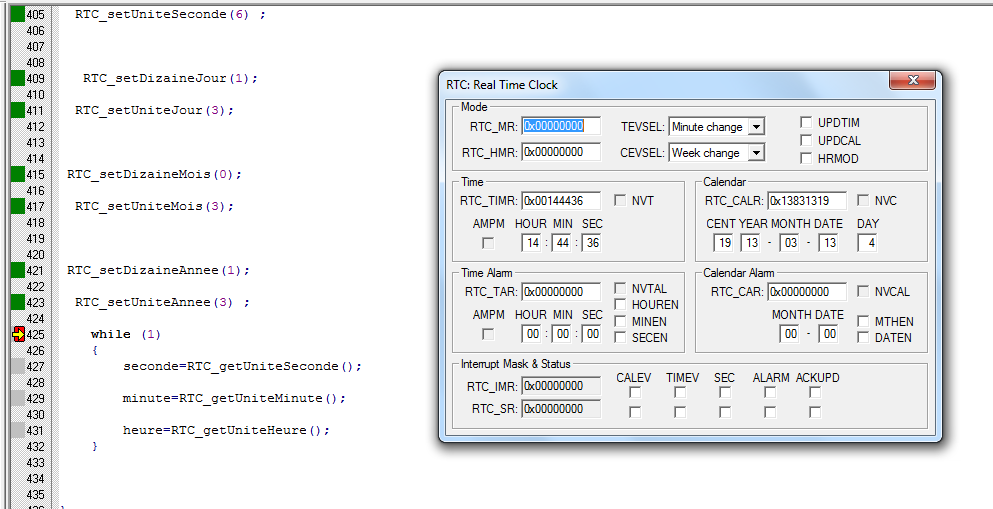
\includegraphics[scale=0.4]{images/RTC_fig1.png}
	\caption{bon fonctionnement des fonctions <<set>>}
	\label{RTC-image1}
\end{figure}

\begin{figure}[h!]
	\centering
	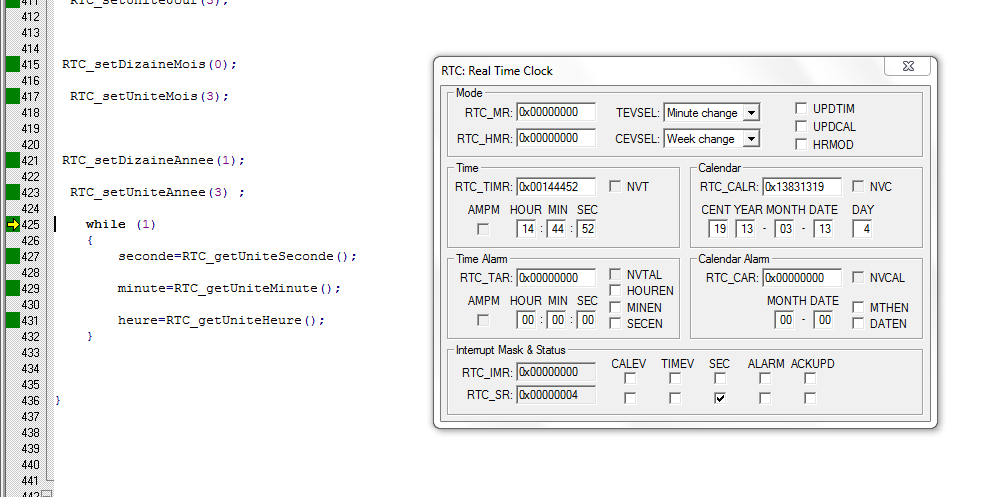
\includegraphics[scale=0.4]{images/RTC_fig2.png}
	\caption{l'horloge compte correctement}
	\label{RTC-image2}
\end{figure}

Puis, ne pouvant tester mon code sur la carte puisque l'écran ne fonctionnait pas encore correctement, j'ai aidé Fabien à concevoir les foncions permettant la production d'une note de musique.
J'ai notamment apporté une importante contribution à la réalisation des fonctions générant les différents <<bip>> ainsi qu'à l'écriture de fonctions d'interruption.

Lorsque j'ai pu tester mon code sur la carte, je me suis aperçu que les fonctions de mise à jour ne fonctionnaient pas correctement. En effet, la modification des valeurs de \texttt{RTC\_TIMR} ne s'effectuait que lorsqu'on exécutait le programme pas-à-pas.
J'en ai donc déduit qu'un temps d'attente était nécessaire au moment de la modification d'une valeur.
Il fallait attendre que le bit \texttt{ACKUPD} du registre SR passe à 1 avant d'écrire dans \texttt{RTC\_TIMR}, ce qui pouvait prendre un certain temps.
J'ai donc dans un premier temps voulu mettre une boucle \texttt{while (!(RTC\_SR \& RTC\_ACKUPD))}.
Cependant, cela n'a pas fonctionné et j'ai donc fait une boucle incrémentant un compteur jusqu'à 4 200 000 afin de produire une attente suffisamment longue.

Cela a bien fonctionné, mais le temps d'attente étant très long, j'ai du changer mes fonctions <<set>> de manière à n'effectuer qu'une seule fois le changement du bit SR, puis modifier toutes les valeurs de \texttt{TIMR} et ensuite réactiver le décompte de la RTC plutôt que de faire \texttt{RTC\_MR = RTC\_UPDTIM} pour chaque fonction <<set>>.

\section{Possibilités d'amélioration}
Pour l'instant, le réglage de l'heure et de la date ne peut se faire que du coté programmeur.
Il aurait été appréciable que l'utilisateur puisse lui aussi mettre à jour l'heure et la date, ou au moins lui laisser la possibilité de choisir entre heure d'été et heure d'hiver.
Cela aurait alors nécessité une collaboration avec la personne chargée de l'affichage et celle chargée de la télécommande.


\part{La pluviométrie\\-\\Yannick \bsc{Larvor}}
\section{Introduction}
Dans une station météo, il est nécessaire de connaître la quantité de pluie qui s’est écoulée sur un instant.
Cette partie va illustrer la programmation d’un compteur de pluviométrie.
\section{Cahier des charges}
\subsection{Objectif à atteindre}
L'objectif de cette partie du projet est d’effectuer la mesure d’une quantité d’eau sur un intervalle de temps et la possibilité de voir son évolution sur un afficheur LCD.
\subsection{Fonctionnement du pluviomètre}
Pour mesurer la quantité de pluie, nous avons à disposition deux augets. L’eau va rentrer dans l’un des deux augets.

\begin{center}
	
\includegraphics[scale=0.4]{images/PLUV_fig1.png}
\end{center}

A partir d’une certaine quantité d’eau, les deux augets vont basculer.
Celui qui est rempli va se vider tandis que celui qui est vide va se remplir.

\begin{figure}[h!]
	\centering
	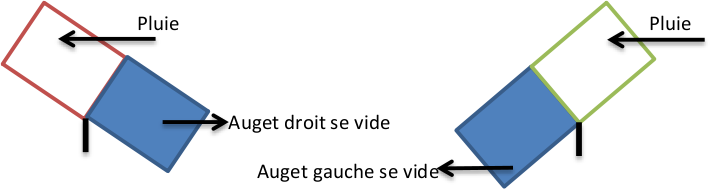
\includegraphics[scale=0.4]{images/PLUV_fig2.png}
	\caption{Auguet droit rempli / Auget gauche rempli\label{PLUV-fig2}}
\end{figure}

La détection du basculement se fait à l’aide d’un aimant. Selon le nombre de basculements et le volume d’un auget, on peut déduire la quantité de pluie écoulée sur un instant t.

\subsection{Gestion du pluviomètre sur un microcontrôleur}
Le calcul de la quantité de pluie est géré par le microcontrôleur.
Comme nous avons vus précédemment, la quantité de pluie est calculée par la relation :
\[
\mbox{Quantité de pluie } = \mbox{ Nombre de basculements des augets } * \mbox{ volume d’un auget}
\]

Afin de simuler un basculement, nous allons utiliser un bouton poussoir sur une entrée du microcontrôleur.
Quand le bouton est inactif, la tension d’entrée est de +5V. La détection d’un appui fait passer sa tension à 0V.

\begin{center}
	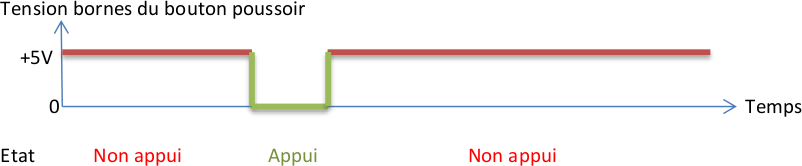
\includegraphics[scale=0.4]{images/PLUV_fig3.png}
\end{center}

Afin d’ajouter d’autres fonctionnalités au pluviomètre, il est souhaitable de remettre à zéro le compteur et connaître la date de la dernière mise à jour de la quantité.
Pour cela, il faut faire appel aux programmes gérant l’afficheur LCD (affichage de la quantité de pluie et/ou date de la dernière mise à jour) et la RTC (configuration de la date).

\section{Programmation du pluviomètre}
Afin d’effectuer la programmation du pluviomètre, plusieurs étapes sont nécessaires.
\subsection{Fonctions}
Pour bien découper le programme et le rendre plus accessible dans le programme principal, il faut réaliser plusieurs fonctions :
\paragraph{Initialisation du bouton poussoir sur le microcontrôleur :}
il faut choisir la broche à relier sur le microcontrôleur.
Le choix s'est porté sur le port B broche 3 car elle est interruptible (IRQ4) et est directement reliée à l'AIC.
Cette fonction permet de configurer la broche comme entrée et d’autoriser une interruption sur celle-ci.
\begin{itemize}
\item Prototype : \texttt{PLUV\_init\_PIOB ();}
\end{itemize}
\paragraph{Configuration de l’AIC gérant l’interruption sur l’état du bouton poussoir :}
le déclenchement d’une interruption se fera sur front descendant de l’état du bouton poussoir.
\begin{itemize}
\item Prototype : \texttt{PLUV\_init\_AIC();}
\end{itemize}
\paragraph{Interruption lors de la détection de l’appui sur le bouton poussoir :}
appel à une fonction faisant la mise à jour de la quantité de pluie.
\begin{itemize}
\item Prototype : \texttt{\_\_irq void PLUV\_interruption\_etat\_switch(void) ;}
\end{itemize}
\paragraph{Calcul de la quantité de pluie :}
fonction qui permet de retourner la valeur de la pluviométrie en cours d’exécution.
\begin{itemize}
\item Prototype : \texttt{PLUV\_getPluviometrie(void);}
\end{itemize}
\paragraph{Mise à jour de la quantité de pluie}
\begin{itemize}
\item Prototype : \texttt{PLUV\_setPluviometrie(void);}
\end{itemize}
\paragraph{Réinitialisation de la quantité de pluie (mettre la pluviométrie à 0)}
\begin{itemize}
\item Prototype : \texttt{PLUV\_clearPluviometrie(void);}
\end{itemize}
\paragraph{Connaître la date de la dernière mise à jour}
\begin{itemize}
\item Prototype : \texttt{PLUV\_getHeureClear(void);}
\end{itemize}

\subsection{Variables globales}
Pour la lecture des éléments calculés dans les différentes fonctions du pluviomètre, il nous faut des variables globales.

\paragraph{Valeur de la quantité de pluie (dernière mise à jour) :}
\begin{itemize}
\item \texttt{int pluviometrie;}
\end{itemize}
\paragraph{Date de la dernière mise à jour :}
\begin{itemize}
\item \texttt{char pluvHeureClear[6]}
\end{itemize}

\subsection{Structure des fichiers de programmation}
Pour la programmation du pluviomètre et l’utiliser par la suite dans le programme principal de la station météo, il faut structurer le programme sous deux fichiers différents.
\begin{itemize}
\item Un fichier \emph{pluviometre.h} qui va regrouper les différents prototypes de fonctions et les différentes variables globales définies en \texttt{extern}.
\item Un fichier \emph{pluviometre.c} qui code les prototypes des fonctions.
\end{itemize}

\section{Validation de la simulation}
Pour valider le fonctionnement du programme en simulation, il faut voir la variable \emph{pluviometrie} varier de 10 en 10 (volume d’un auget) à chaque front descendant de la broche 3 du PIOB.

\begin{figure}[h!]
	\centering
	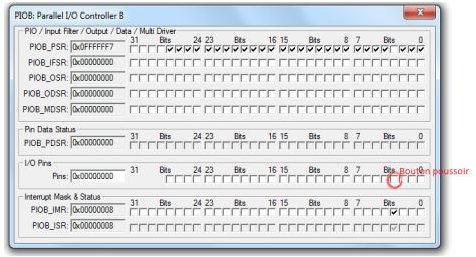
\includegraphics[scale=0.6]{images/PLUV_fig4.jpg}
	\caption{Configuration du bouton en simulation\label{PLUV-fig4}}
\end{figure}

Les résultats de simulation montrent bien que le compteur de pluviométrie s’incrémente à chaque cochage (+5V) décochage (0V) sur l’entrée PB3.

\section{Validation sur la carte}
Cette partie va présenter le câblage d’un bouton poussoir sur la carte de test.
L' objectif est de voir un passage à 0V lors d’un appui et de rester à +5V sans appui.
Pour cela, le schéma suivant a été implanté sur la carte :

\begin{figure}[h!]
	\centering
	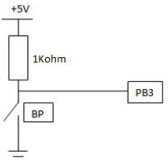
\includegraphics[scale=0.9]{images/PLUV_fig5.jpg}
	\caption{Schéma de câblage du bouton poussoir sur la carte\label{PLUV-fig5}}
\end{figure}

Pour vérifier la validité du fonctionnement, il suffit de voir incrémenter la valeur de la pluviométrie sur l’afficheur LCD à chaque appui sur le bouton.
Les résultats ont validé les objectifs attendus.

\section{Conclusion}
La mesure de la pluviométrie est fonctionnelle en simulation et sur la carte.
Le stockage de l’heure de la dernière mise à jour n’a pas été testé.

Les principales difficultés dans la programmation de la partie pluviométrie a été la gestion de l’interruption et les problèmes du logiciel dans la simulation.
À partir de ce projet, j’ai pu en apprendre davantage dans la programmation du PIO et avoir des notions dans le débuggage d’un programme.

\part{La température\\-\\Yannick \bsc{Riou}}
Dans le cadre du projet de réalisation d'une station météo, il est demandé de pouvoir relever la température grâce à un capteur analogique de référence LM35.
Ce document présente l'étude et l'implémentation du capteur pour notre projet.
\section{Capteur LM35}
Le capteur LM35 est un capteur de température analogique qui délivre une tension proportionnelle à la température. La correspondance donnée dans la documentation est : 10 mV / $^\circ$C.

Ce capteur peut être utilisé pour mesurer des températures positives mais on peut aussi le câbler pour qu'il soit en "Full-Range" (pleine échelle) et pouvoir ainsi mesurer des températures négatives et positives.  L'étude qui suit porte sur le LM35 qui peut mesurer des températures négatives, or notre composant est le LM35DZ dont la plage est +0 $^\circ$C à 100 $^\circ$C.
Pour cela il est nécessaire de modifier le circuit.

\begin{figure}[h!]
	\centering
	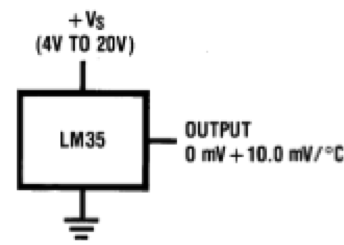
\includegraphics[scale=0.6]{images/TEMP_fig1.png}
	\caption{Capteur $+2^\circ C$ à $+150^\circ C$}
	\label{TEMP-fig1}
\end{figure}

Ce montage (figure \ref{TEMP-fig1}) est donc le capteur seul, on en peut  que mesurer des températures entre +2 $^\circ$C et +150 $^\circ$C. Or nous souhaitons pouvoir au moins détecter des températures de l'ordre de -5 $^\circ$C  à -10 $^\circ$C.

On fournit donc au LM35 une tension négative :

\begin{figure}[h!]
	\centering
	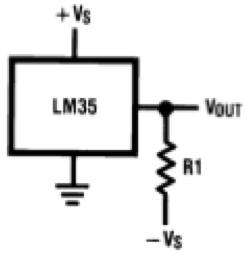
\includegraphics[scale=0.6]{images/TEMP_fig2.png}
	\caption{Capteur $-55^\circ C$ à $+150^\circ C$}
\end{figure}

Grâce à ce montage, en choisissant la résistance R1 = -Vs/50$\mu$A où Vs est l'alimentation négative, on obtient des équivalences  avec un facteur 10 entre température et voltage : 1500 mV pour +150 $^\circ$C et -550 mV pour -55 $^\circ$C.

Même si générer une tension négative n'est pas si compliqué, grâce à un amplificateur opérationnel inverseur par exemple, il existe un troisième montage qui permet de se passer d'une alimentation négative :

\begin{center}
	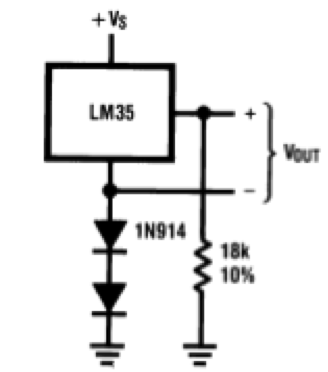
\includegraphics[scale=0.6]{images/TEMP_fig3.png}
\end{center}

Les deux diodes 1N914 possèdent chacune une tension en direct de 0,75 V, on retrouve donc 1,5 V sur la borne "-" de Vout.
La résistance de 18k$\Omega$ est une résistance dite de "pull-down", elle force la borne "+" de Vout à la masse.
Si à la sortie du LM35 on à 0 V, cela veut dire que l'on a une température négative.
Vout vaut donc Va = 0 -  1500 mV, or la précision du capteur est de 10 mV/ $^\circ$C, on a donc une température de -150 $^\circ$C.
Plus Vs (sortie du LM35) va augmenter et plus "Va" augmentera vers des températures positives.

On obtient donc un capteur qui peut détecter des températures positives et négatives.

Comme nous avons pu le voir le capteur LM35 est analogique, pour pouvoir traiter et afficher la température sur notre carte de développement il faut convertir cette tension en un nombre exploitable numériquement.
Nous avons besoin d'un convertisseur analogique numérique. Sachant qu'un ADC ne peut pas lire une tension négative, il reste encore à résoudre le problème de la tension négative délivrée par le LM35 pour des températures négatives. Cette étude n'est finalement pas nécessaire car le composant que nous utilisons LM35DZ ne peut mesurer que des températures entre 0 et +100 $^\circ$C. Elle permet quand même de se rendre compte de ce qu'il faut mettre en place pour pouvoir lire des températures négatives avec un capteur analogique.

\section{Convertisseur Analogique Numérique (ADC)}
La carte de développement que nous allons utiliser pour construire notre station météo est articulée autour d'un AT91M55800A produit par ATMEL avec un coeur ARM. Il possède 2 modules ADC de 4 channels chacun.

\section{Configuration sur l'ATM88500A}

\begin{figure}[h!]
	\centering
	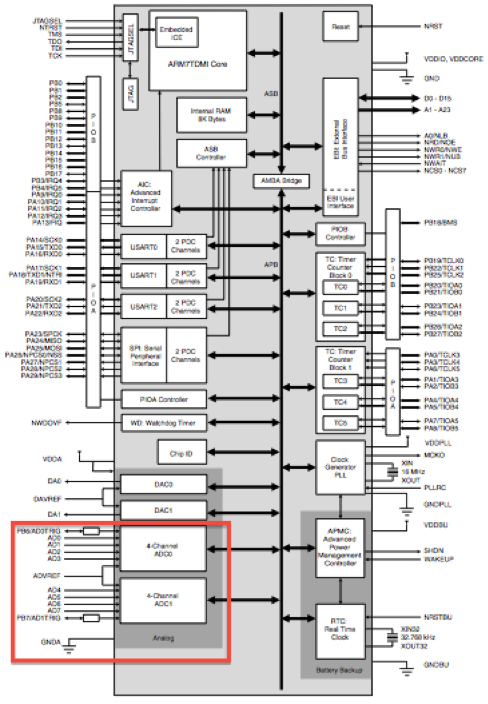
\includegraphics[scale=0.6]{images/TEMP_fig4.png}
	\caption{Bloc diagramme du ATM88500A}
\end{figure}

Nous allons utiliser pour notre application le module ADC0 et le channel 0. Pour pouvoir utiliser le périphérique, il faut le configurer. La procédure et les registres concernés sont les suivants :

\begin{itemize}
\item On commence par alimenter le périphérique grâce au registre \texttt{APMC\_PCER}.
\item On configure le registre \texttt{ADC0\_MR}, qui permet de choisir le mode de fonctionnement. Dans notre cas, on choisit de lancer la conversion de façon logicielle, c'est à dire quand l'utilisateur aura appuyé sur la télécommande. La conversion sera faite sur 10 bits qui est une résolution raisonnable. Enfin le module est mis en mode "normal" (à l'inverse du mode "sommeil" qui permet d'économiser de l'énergie).
\item On active ensuite le channel correspondant, pour nous le channel 0.
\item On désactive les interruptions de fin de conversion et les masques d'interruptions.
\item L'acquisition de la valeur se fait ensuite en remplissant le registre \texttt{ADC0\_CR} avec le flag \texttt{ADC\_START}. On attend la fin de conversion en scrutant le bit n $^\circ$1 du registre \texttt{ADC0\_CR}. Quand celle-ci est terminée, le mot de 10 bits est disponible dans le registre \texttt{ADC0\_CDR0}.
\end{itemize}

Nous allons maintenant fournir l'étude pour pouvoir interpréter le nombre reçu grâce à la conversion, par rapport à la tension lue et enfin le lier avec la température réelle.

\section{Étude théorique et interprétation}
Le mot fourni par le convertisseur analogique numérique va de 0 à 1023 (10 bits). Sachant que le capteur et l'AT91M55800A sont alimentés en 3.3 V, la sortie du capteur de température varie de 0 V à 3.3 V. Le quantum, ou plus petite variation mesurable par le convertisseur, est donné par

\[
q = {P.E \over 2\up{10}-1} = {3.3 \over 1023} = 3.22 mV
\]

Or notre capteur bouge de 10 mV/ $^\circ$C. On en déduit que quand le capteur augmente d'un degrés Celsius (10mV), le nombre en sortie du convertisseur augmente de 3,099 (10 mV $\approx$ 3,099 $\times$ 3,22 mV). On a donc l'équivalence suivante entre la température lue et le nombre en sortie du convertisseur :

\[
T(^\circ C) = {nbConvertisseur \over 3,099}
\]

\begin{center}
	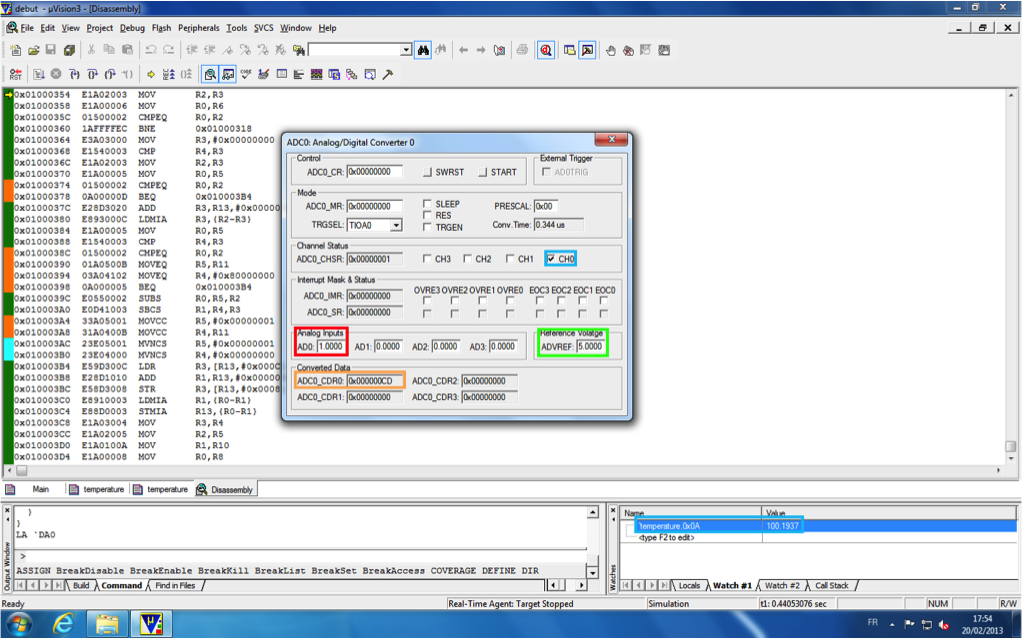
\includegraphics[scale=0.6]{images/TEMP_capture.png}
\end{center}

On valide le fonctionnement du programme en simulation.

En bleu, on peut voir que la configuration a bien été prise en compte car le channel 0 est coché. En rouge on entre la valeur analogique, après avoir renseigné la tension de référence, ici 5V (en vert), finalement la tension de référence s'avère être 3.3V. On obtient en sortie une valeur en hexadécimal, ici 0xCD soit 205 en décimal pour la tension de référence de 5v et 0x136 soit 310. On remarque que en bas à gauche on obtient la valeur de la température contenue dans une variable. Le calcul pour obtenir la variable température est celui donné plus haut. On peut vérifier que cela fonctionne car si en entrée on a 1 V (1000 mV), cela donne 100 $^\circ$C.

Le schéma électrique à réaliser sur plaque est donc simple, alimenter le LM35DZ avec une tension de 3.3 V et le connecter sur l'entre ADC0 du microcontrôleur.
Il reste maintenant à faire le circuit sur plaque d'essai et tester avec le microcontrôleur.

\section{Organisation du programme}
Le programme s'organise en 3 fonctions principales :
\begin{itemize}
\item Fonction d'initialisation du convertisseur analogique numérique
\item Fonction de conversion et de calcul de la température
\item Fonction de retour de la température
\end{itemize}

\section{Tests}
Nous avons essayé premièrement de mettre une tension sur l'entrée du convertisseur, cela sans succès, la valeur restant bloquée sur un nombre fixe. Même en essayant de changer de channel, cela n'a rien changé.

Cela vient donc soit de l'entrée de l'ADC qui est défectueuse ou de l'AOP en suiveur qui est détruit.

\section{Conclusion}
Ce projet fut donc très enrichissant car il a permis de mettre en oeuvre un microcontrôleur ARM, architecture qui est très répandue. Le plaisir a un peu été gâché par des disfonctionnements incompréhensibles. Malgré cela, nous avons pu travailler en équipe sur un sujet intéressant.


\part{La télécommande\\-\\Adrien \bsc{Coudray}}
\section{Codage RC5 – démarche de décodage}
\subsection{Codage RC5}
La trame reçue par le processeur est de type RC5. Ce code est basé sur le codage manchester.
C'est à dire qu'un bit est codé sur deux états : un état bas suivi d'un état haut pour le '1' et l'inverse pour le '0'.

Voici un exemple de code RC5 :

\begin{center}
	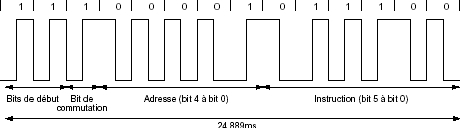
\includegraphics[scale=0.6]{images/RC_rc5.png}
\end{center}

Le code commence par deux bits de début, à '1', suivi d'un bit de commutation.
Ce bit de commutation indique si la trame précédente est identique ou non à la trame courante.
Ensuite, on a l'adresse du périphérique qui a envoyé la trame, sur 5 bits.
Enfin, on a l'instruction sur 6 bits.

La durée d'une trame est de 24,889 ms, on a donc une période de 1,778 ms et une demi période de 0,889 ms.

Ce que l'on peut remarquer, c'est que si on échantillonne cette trame sur une période 2 fois plus petite, donc sur une fréquence deux fois supérieure, on obtient une trame avec 2 fois plus de bits.

Par exemple <<1010>> codé en manchester donne <<01100110>>.
Si on récupère la trame complète, on peut facilement retrouver le code originel en prenant un bit sur deux.
On procédera de la même manière pour le projet.

\subsection{Démarche de décodage}
Voici le principe de fonctionnement du décodage de la trame :

\begin{center}
	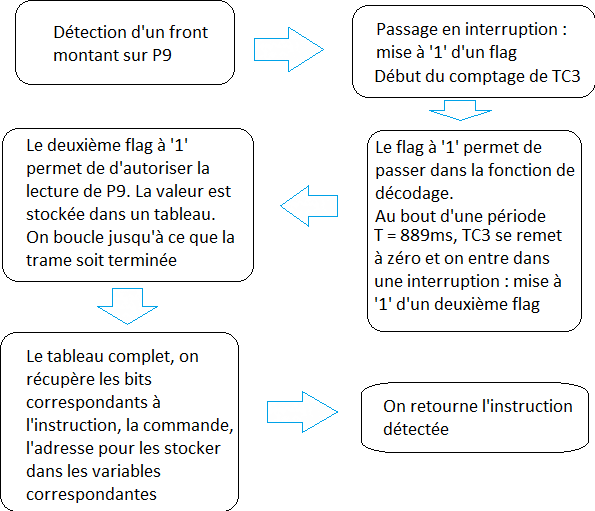
\includegraphics[scale=0.4]{images/RC_diagramme.png}
\end{center}

Cette approche fonctionne parfaitement en simulation.
En pratique nous avons eu des soucis concernant les buffers qui étaient défectueux et qui ne permettaient pas l’application.

\section{Le codage en C}
Pour plus de détails, le code est entièrement fourni en annexe.
Nous allons nous intéresser ici au rôle des fonctions.

\subsection{Les fonctions d’initialisation}
\begin{itemize}
\item \texttt{RC\_initTC3}
\end{itemize}
Cette fonction permet de paramétrer le timer counter TC3.
La configuration choisie est la suivante :
mode capture, reset du compteur si on atteint la valeur de RC, horloge de 1Mhz et l’alimentation.
La valeur de RC est de 889 (qui correspond à la période d’échantillonnage du signal).
\begin{itemize}
\item \texttt{RC\_initPIOA}
\end{itemize}
L’initialisation du PIOA permet de paramétrer l’E/S P9 en entrée et d’autoriser une interruption sur celle-ci.
On paramètre également son alimentation.
\begin{itemize}
\item \texttt{RC\_initAIC\_P9}
\end{itemize}
Cette fonction gère la gestion de l’interruption sur P9 au niveau de l’AIC.
Elle consiste en fait à activer une interruption sur niveau haut puis à attribuer la fonction qui sera appelée en cas de détection d’interruption.
La priorité attribuée est la plus haute.
\begin{itemize}
\item \texttt{RC\_init\_TC3}
\end{itemize}
De même que la fonction précédente, cette fonction paramètre une interruption : celle de TC3, qui se déclenche lorsque TC3 atteint la valeur de RC.
Il s’agit, à la différence de la fonction précédente, d’une interruption interne.
La priorité est également maximale.

\subsection{Les fonction d’interruptions}
\begin{itemize}
\item \texttt{\_\_irq void RC\_interruption\_PIOA}
\end{itemize}
Cette première fonction d’interruption est appelée lors de la détection d’un niveau haut sur P9.
Elle a deux rôles importants : lancer le comptage de TC3, mettre un flag à ‘1’ pour indiquer la détection.
Enfin elle est désactivée pour éviter qu’elle ne se relance lors du prochain niveau haut, qui arrivera au prochain bit à ‘1’ de la séquence RC5.
\begin{itemize}
\item \texttt{\_\_irq void RC\_interruption\_TC3}
\end{itemize}
La seconde fonction d’interruption a pour rôle d’indiquer lorsque TC3 a atteint la valeur de RC.
La première ligne va lire le bit d’indication d’interruption (qui se met à ‘1’ en cas d’interruption sur TC3 détectée) du registre de statut de TC3.
Cette ligne est nécessaire, car sans cela, aucune nouvelle interruption sur TC3 n’est possible.
La suite consiste simplement à mettre un nouveau flag à ‘1’.

\subsection{La fonction de décodage}
\begin{itemize}
\item \texttt{int RC\_get\_code}
\end{itemize}
Fonction la plus importante du programme, elle gère la récupération de la trame ainsi que son décodage.
Elle fonctionne de la manière suivante : on boucle tant que la trame n’est pas entièrement récupérée.
Pour indiquer qu’un bit de la trame est récupéré, on attend l’interruption du compteur qui va mettre un flag à ‘1’, ce qui va permettre de rentrer dans le <<if>> qui va charger la valeur de P9 dans un tableau.
Cela fait, on incrémente l’indice ‘i’.
Cela est répété 30 fois afin de récupérer la trame entière et éventuellement vérifier qu’on a bien terminé la récupération de la trame (il suffira pour cela de regarder les derniers bits du tableau créé).
Une fois la trame complète récupérée, le décodage est simple.
Il suffit de prendre un bit sur deux.
Comme on peut le remarquer, j’ai un bit de décalage avec celui que je devrais prendre au premier abord.
Cela s’explique par le fait que le premier bit à ‘1’ sert en fait à la détection de la trame qui va lancer le TC3.
Une fois le premier comptage effectué, le bit est <<perdu>> et on récupèrera le suivant, un ‘0’ donc.
Il ne faut donc pas prendre les bits pairs, mais bien impairs, pour pouvoir décoder la trame.

\section{Simulation}
Dans cette partie nous allons étudier le fonctionnement de la détection d’une trame pas à pas.

\begin{center}
	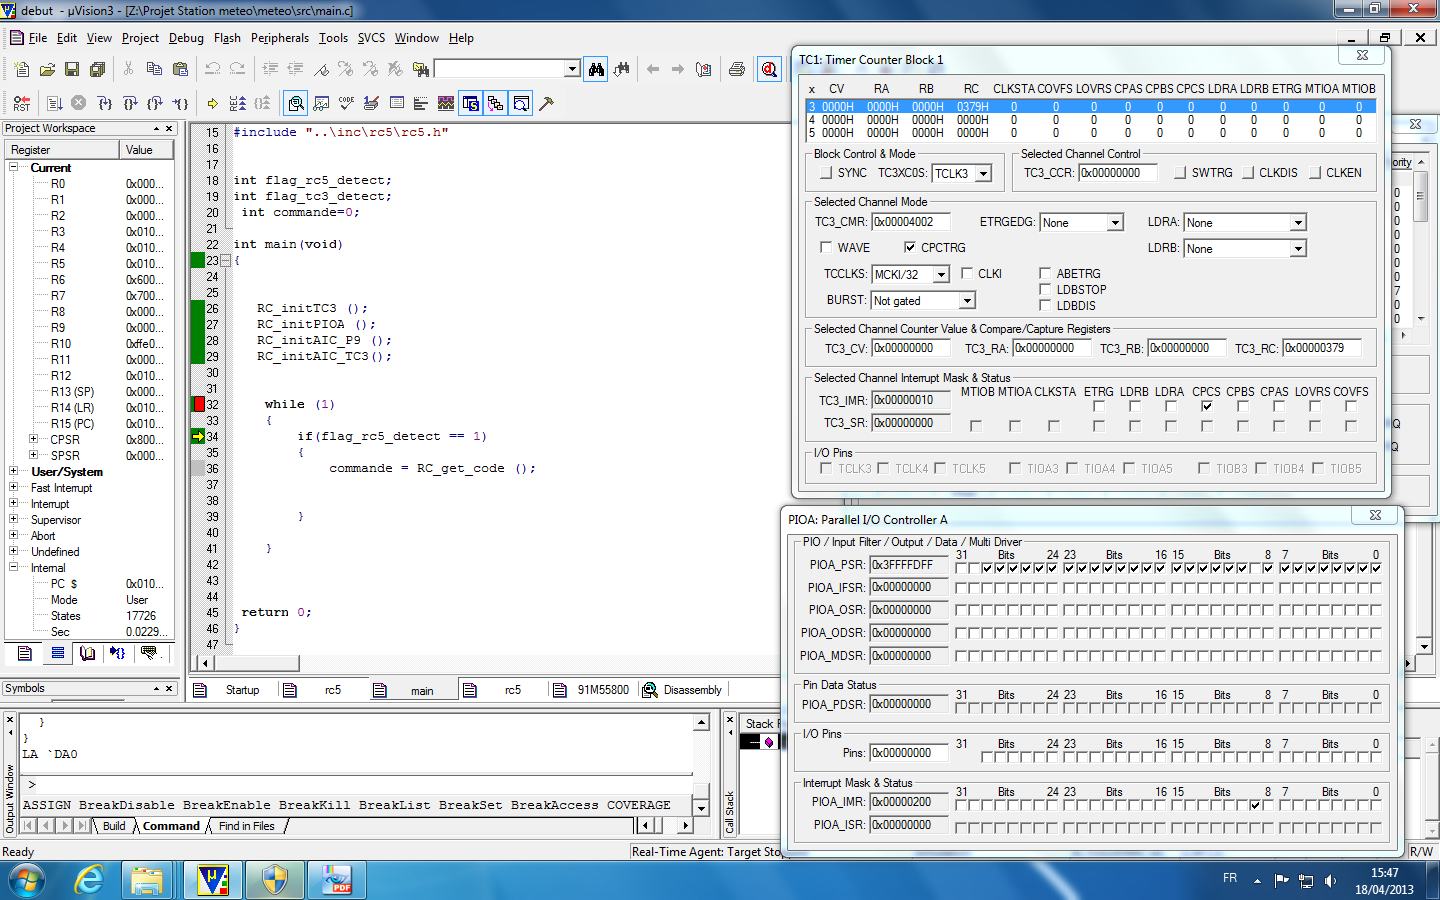
\includegraphics[scale=0.3]{images/RC_simu1.png}
\end{center}

Cette capture d’écran correspond au début de la simulation.
Avec un main fait pour la simulation, on procède à l’initialisation des PIOA, TC3 et interruptions.
Ensuite une boucle va tester le \texttt{flag\_rc5\_detect} qui passera à ‘1’ si on détecte un niveau haut sur P9, ce qui a été fait dans la capture suivante :

\begin{center}
	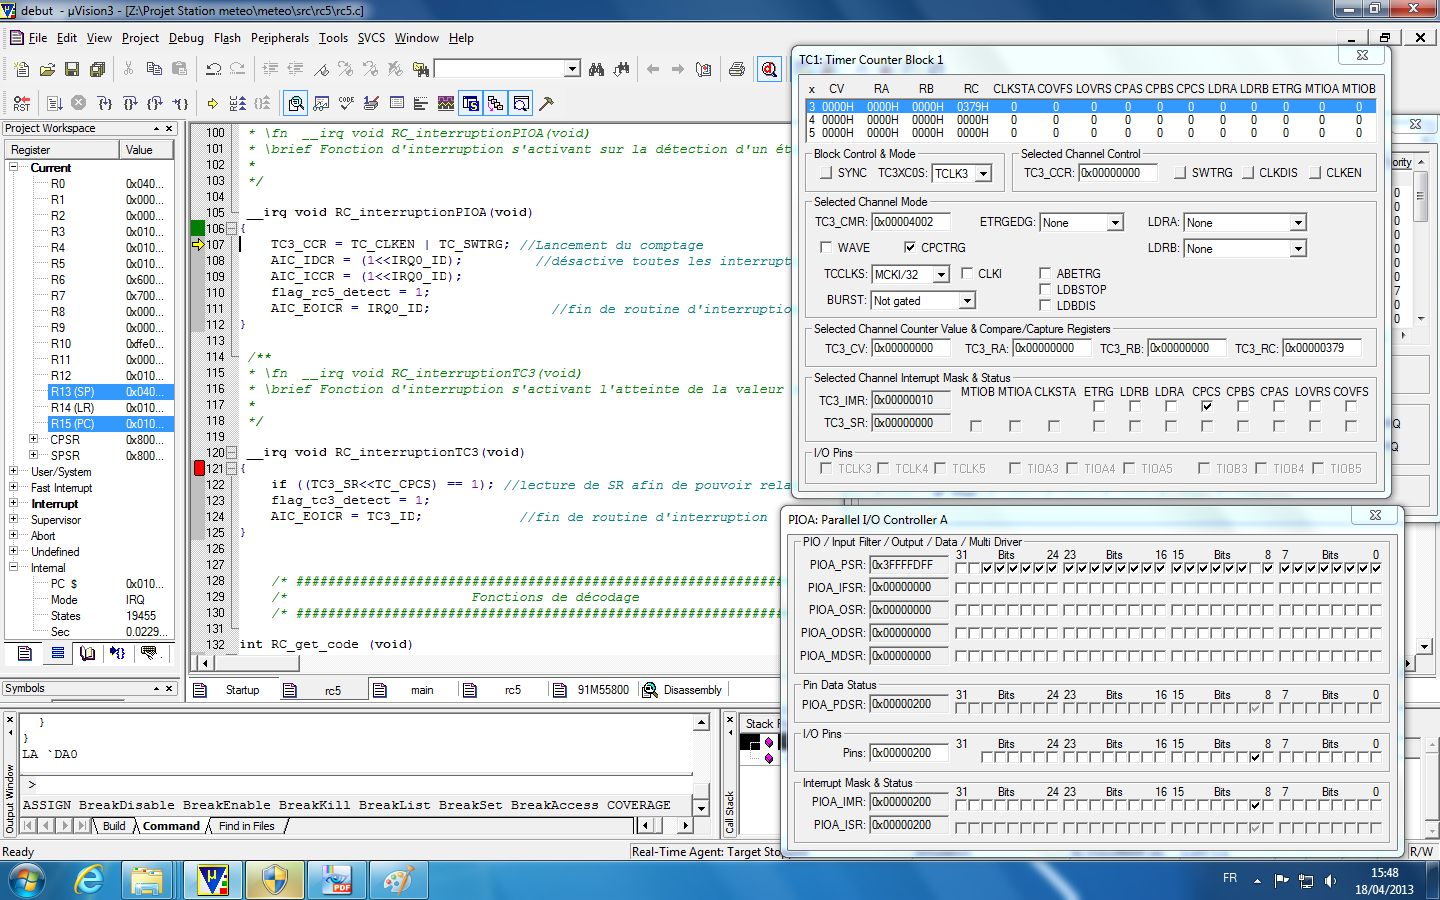
\includegraphics[scale=0.3]{images/RC_simu2.png}
\end{center}

Ici on peut voir sur la fenêtre de droite que l’on a mis le bit n$^\circ$9 du PIOA à ‘1’, ce qui correspond à un niveau haut sur P9.
Cela a bien déclenché l’interruption souhaitée.
Le \texttt{flag\_rc5\_detect} va donc passer à ‘1’ et le comptage de TC3 est lancé.

\begin{center}
	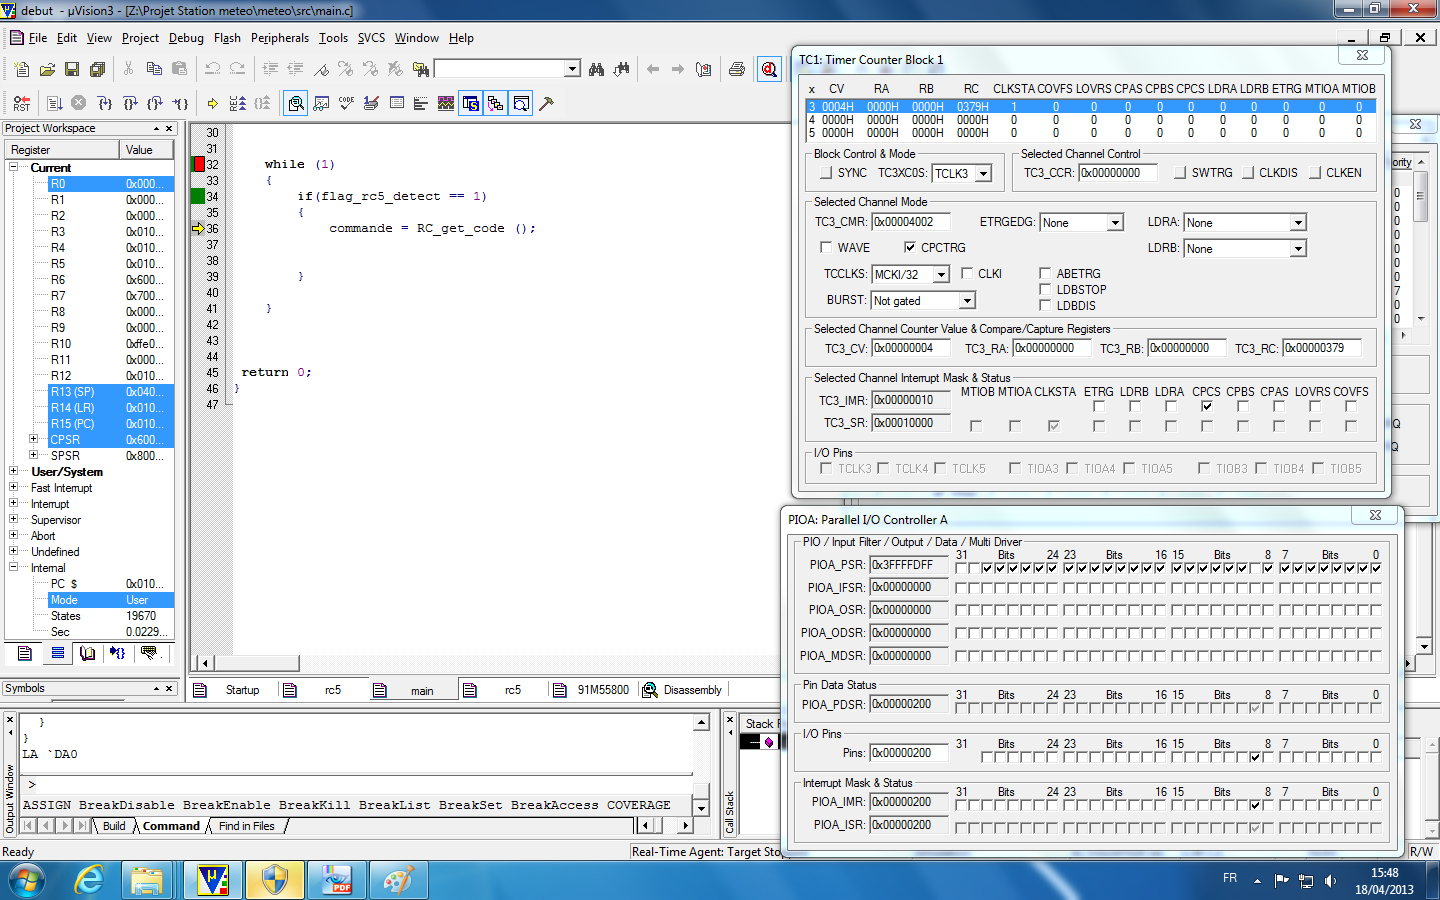
\includegraphics[scale=0.3]{images/RC_simu3.png}
\end{center}

Comme on peut le voir, la mise à ‘1’ du flag s’est bien déroulée, on entre donc dans la fonction \texttt{RC\_get\_code}.
On fait avancer le programme jusqu’à ce qu’on arrive à la boucle qui va tester si le TC3 a atteint la valeur souhaitée.

\begin{center}
	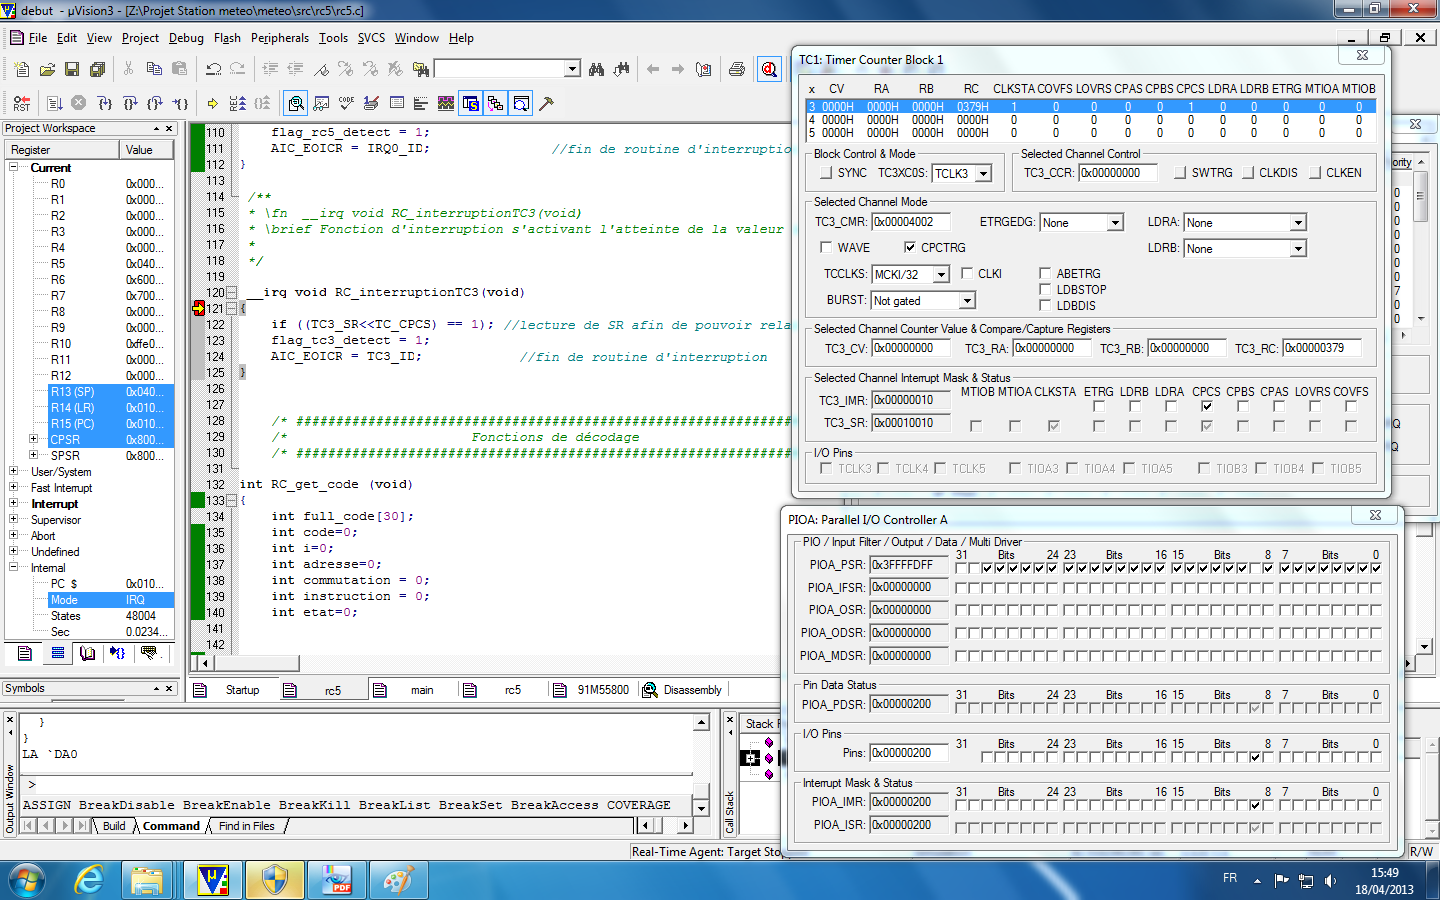
\includegraphics[scale=0.3]{images/RC_simu4.png}
\end{center}

Cette capture montre que l’on entre bien dans l’interruption de TC3, qui va alors positionner le flag correspondant à ‘1’.
On devrait donc par la suite récupérer la valeur de P9 pour la stocker dans un tableau.

\begin{center}
	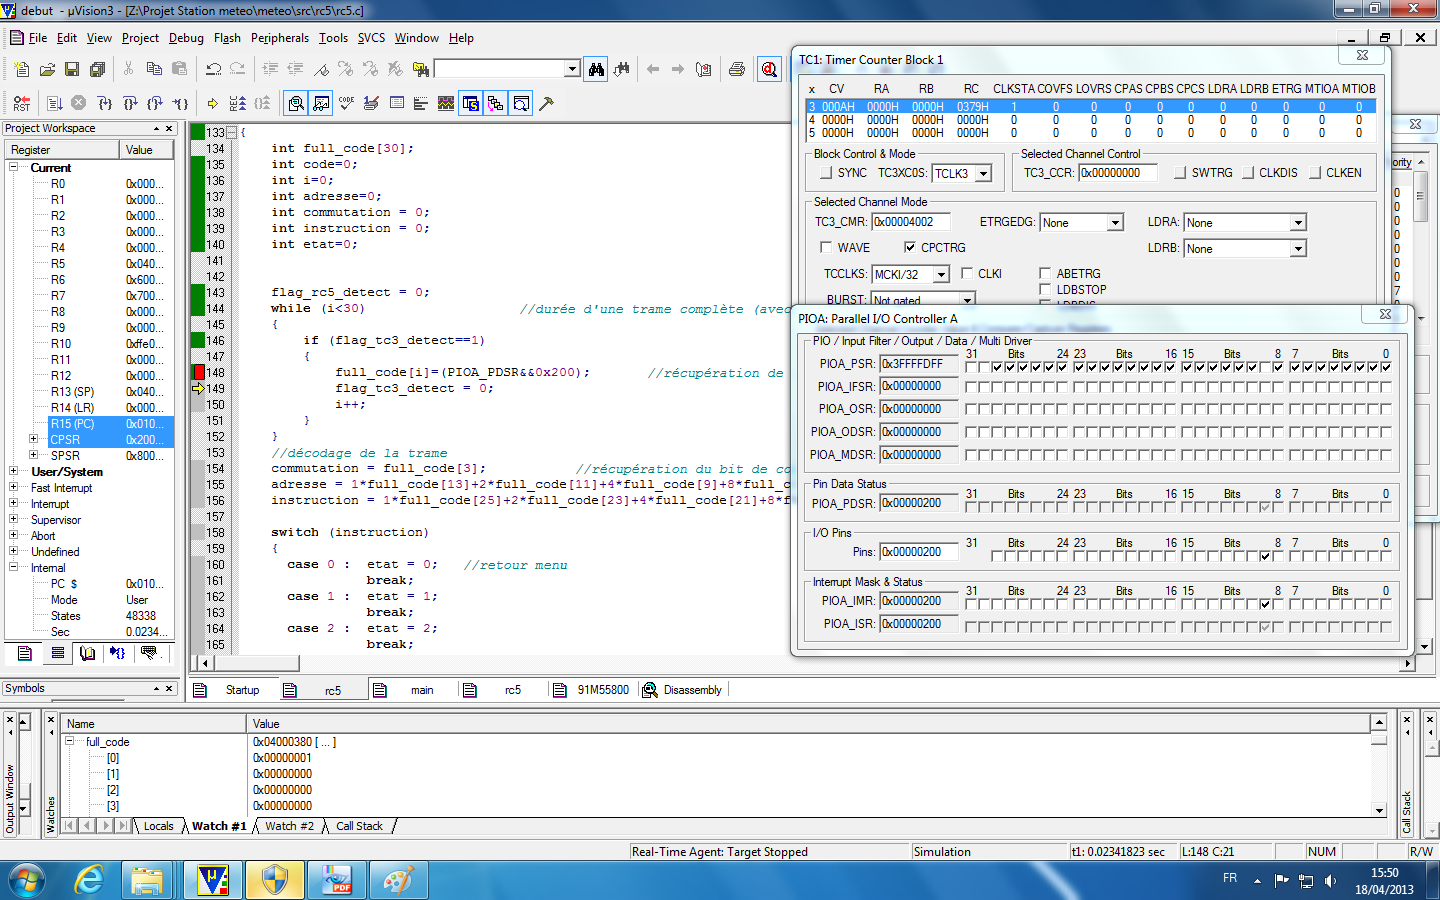
\includegraphics[scale=0.3]{images/RC_simu5.png}
\end{center}

Cette image montre en effet ce cas.
Le programme a été avancé pour montrer que le tableau a bien récupéré la valeur ‘1’ dans sa première case, valeur de P9 comme montré sur la fenêtre de droite.

Nous allons maintenant encore avancer le programme jusqu’à la case 25 du tableau.
Cette case correspond au bit de poids faible de l’instruction, qui sera retournée au programme principale afin d’afficher la température, la pluviométrie etc.
En le plaçant à ‘1’, nous allons vérifier que cette dernière est bien décodée.

\begin{center}
	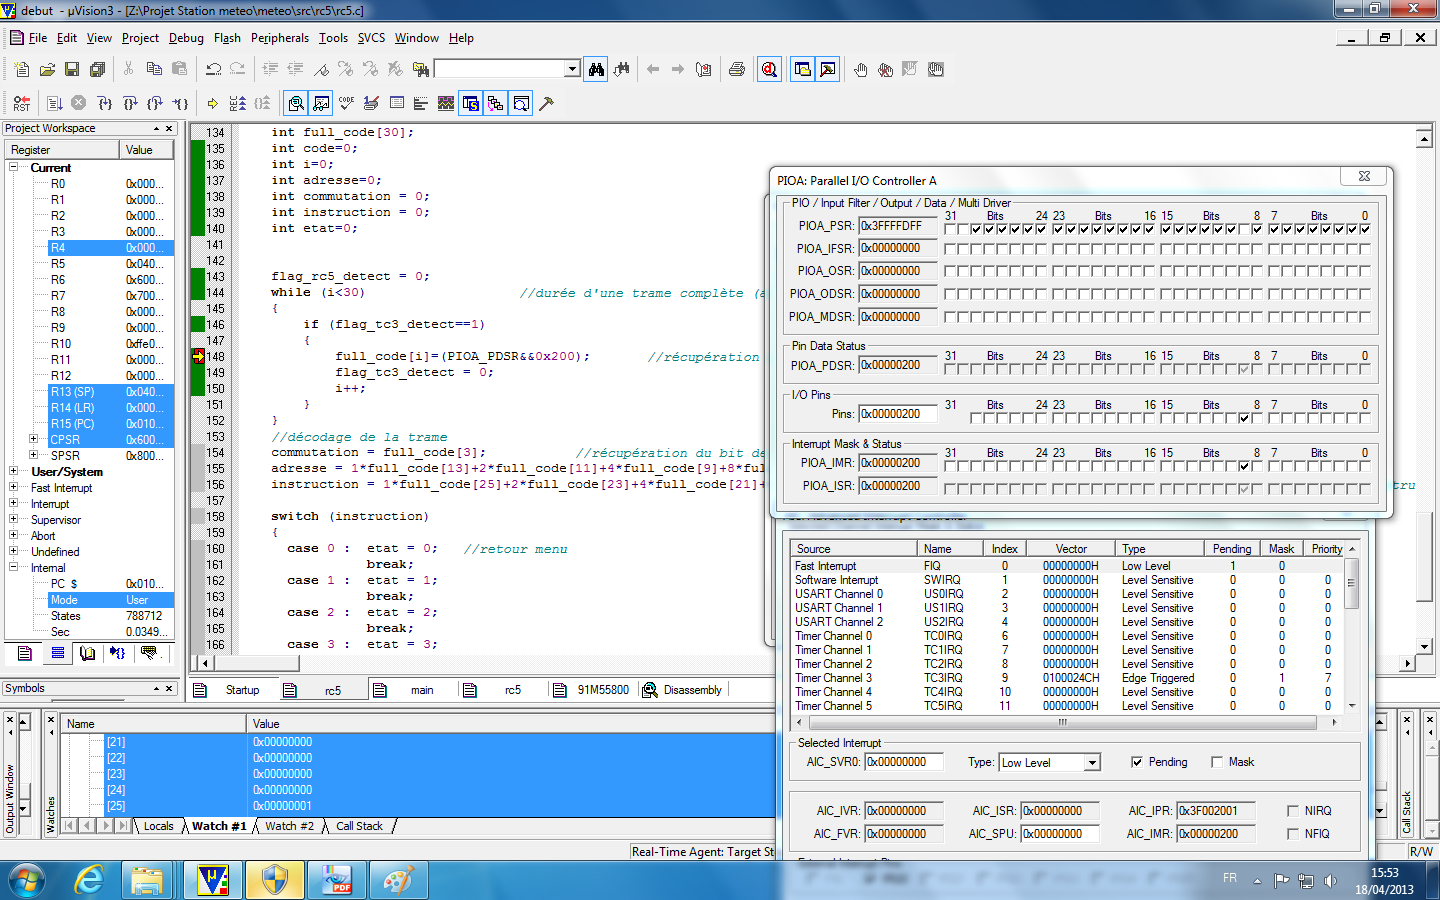
\includegraphics[scale=0.3]{images/RC_simu6.png}
\end{center}

Comme on peut le voir, le ‘1’ a bien été lu sur P9 et la valeur stockée dans la case 25.
Procédons maintenant au décodage :

\begin{center}
	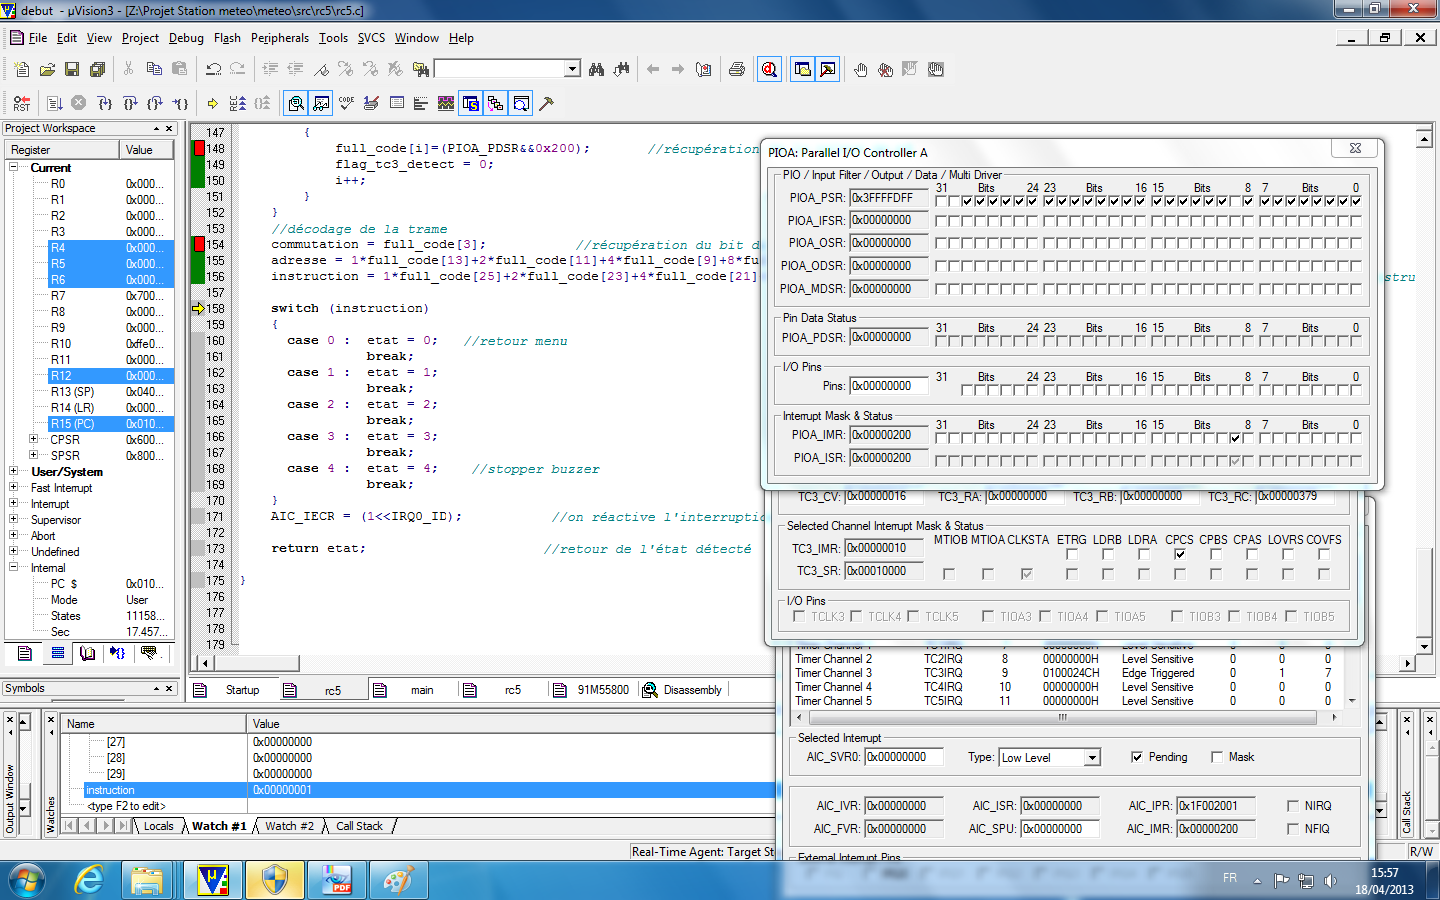
\includegraphics[scale=0.3]{images/RC_simu7.png}
\end{center}

On peut ici voir la valeur de la variable <<instruction>> en bas de l’image qui est l’instruction qui a été décodée de la trame.
Un ‘1’ est bien récupéré et retourné au programme principal.
Pour terminer, on réactive l’interruption sur niveau haut afin d’être prêt à récupérer une nouvelle séquence.

\section{Conclusion}
En conclusion, travailler sur le RC5 fut très intéressant.
J’ai pu ainsi apprendre comment fonctionnait un élément de la vie de tous les jours : une télécommande de télévision.
Cependant, à cause de soucis techniques, notamment à cause des buffers suivi de problèmes de niveaux de tensions lorsque j’ai voulu tester une solution alternative, nous n’avons pu tester le code sur la carte.
Néanmoins les résultats en simulation sont bons et montrent que cette méthode est viable pour décoder le RC5.

Pour aller plus loin, on pourrait envisager la création d’un menu interactif, pilotable avec les touches de la télécommande, ou encore la mise en veille de l’écran pour économiser de l’énergie.
On peut également penser à un contrôle du volume de la carte avec cette télécommande ou bien piloter plusieurs cartes avec la même télécommande :
après l’envoi d’un signal, par exemple en appuyant sur la touche 1, on sélectionnerait la carte 1 et les autres resteraient insensibles à la télécommande jusqu’à ce que l’on ait appuyé sur leur touche attribuée.


\part{L'afficheur LCD\\-\\Jean-Michel \bsc{Nokaya}}
\includegraphics[width=14cm,height=8cm]{images/hello.png}

On m'a assigné la configuration de l'afficheur LCD de la station météo. En effet, cet appareil est essentiel pour l'utilisateur, sans quoi il ne pourrait recueillir les données de manière simple et visible directement. Le masque attribué à mes fonction est LCD\_.

\section{Description de l'afficheur LCD}
\subsection{Description générale}
	 			\paragraph{}
      				L'afficheur LCD à commandes séries est composé d'un écran LCD standard associé à une platine de commande dotée d'un connecteur et d'un câble de raccordement à 3 fil). Ces derniers peuvent être pilotés par un micro-contrôleur doté d'une liaison série (nous utiliserons dans ce projet le modèle AT91M558000), par un compatible PC (avec un circuit intégré MAX-232 additionnel) ou encore par un module "PICBASIC", sans que nous ayons à nous intéresser au fonctionnement proprement dit de l'afficheur.
      			\paragraph{}
      				L'écran LCD à disposition comporte 2 lignes de 16 caractères et n'est pas rétro-éclairé. La vitesse de communication de l'afficheur est fixée à un débit de 19 200 bds.
      	\subsection{Interfaçage avec le micro-contrôleur}
      			\paragraph{Le LCD et la carte}
      				L’interfaçage de l'afficheurs LCD à commandes séries avec le micro-contrôleur doit se faire avec le câble de liaison 3 fils en reliant le fil (rouge) +5V au +5 Vcc d’alimentation (l’alimentation doit être régulé et filtré) et la le fil GND (noir) à la masse du montage. Il faut ensuite relier le dernier fil RX à la sortie du micro-contrôleur.
		%Image à mettre : le schéma de montage
					Néanmoins, il est précisé dans la datasheet du LCD que les signaux de commande doivent être dans la plage [-5V;5V]. Or les signaux envoyés par la carte se trouve dans l'intervalle [-12V;12V]. Et sur l'afficheur il a été ajouté par le concepteur un module qui permet de faire convertir ces signaux à 12V en signaux de 5V. C'est pourquoi nous avons branché le fil qui permet la transmission de commandes et d'informations directement sur ce module, en soudant sur le port ERX du LCD.
				\paragraph{L'USART}
					L'USART ou Universal Synchronous Asynchronous Receiver Transmitter est l'interface qui permet l'échange de données entre la micro-contrôleur et l'afficheur LCD. En effet, le modèle AT91M558000 comporte trois USART, relié au Peripheral Data Controller. L'USART est composé de nombreux registres pour le configurer, et donc pour l'adapter au système auquel on le relie : le LCD ici.

					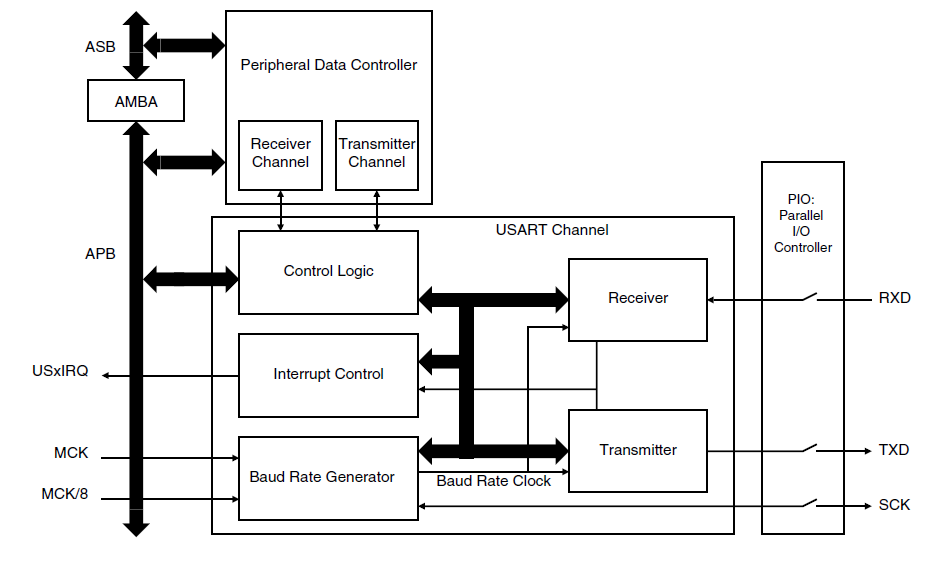
\includegraphics[width=15cm,height=8cm]{images/USART.png}
					\paragraph{\textit{Figure 0.1 : Diagramme en block de l'USART, ATM91558000 Datasheet}}

	\section{Conception du code pour le fonctionnement de l'afficheur LCD}

		\subsection{Démarche}
				\paragraph{L'initialisation}
					On s'est intéressé à la fonction transmetteur de l'USART. C'est pourquoi dans la fonction permettant d'initialiser l'USART (LCD\_INIT\_USART), on a spécifié tous les champs qui autorisent le transmetteur et interdisent l'utilisation du receveur. Ces paramètres sont dans le Control Register (US0\_CR). C'est aussi dans ce registre que nous effectuons les mises à zéro de l'USART, et que nous pouvons lui demander de mettre en place des interruption via le bit (US0\_STTBRK).
					Cette fonction est importante aussi pour le mapping de la carte, en attribuant les broches pour l'alimentation de l'USART0. A l'initial nous utilisions l'USART1, mais nos encadrants ont noté que celui-ci ne fonctionnait pas avec le LCD.

				\paragraph{}
					On initialise l'USART pour qu'il soit fonctionnel avec le LCD. Ainsi, nous avons paramétré via le Mode Register l'enveloppe du signal à envoyer au LCD pour qu'il soit compréhensible par celui-ci. Certaines choses sont à spécifier sur la configuration de ce registre : nous sommes en mode asynchrone, le LCD fonctionne sans horloge, même si le transmetteur a le même comportement dans les deux cas. Par ailleurs, si nous utilisons le mode normal pour l'USART Channel, c'est parce que les autres modes permettent une redirection des canaux entre les broches TXD et RXD de l'USART, rendant la configuration soit du transmetteur, soit du receveur, voire les deux en même temps, tout simplement inutile. Et ce n'est pas ce qu'il nous a été demandé de faire.

					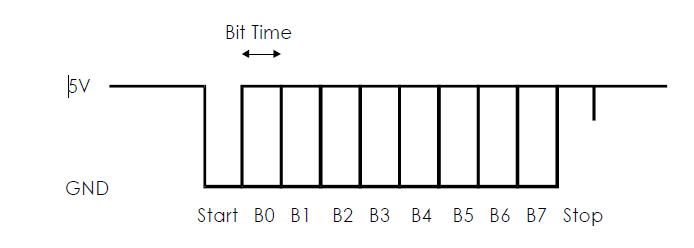
\includegraphics[width=10cm,height=6cm]{images/signauxLCD.png}
					\paragraph{}
					\paragraph{\textit{Figure 0.2 : Signaux compréhensibles par le LCD, ATM91558000 Datasheet}}

				\paragraph{}
					Le modèle de l'afficheur LCD permet un taux d'envoi de 19 200 bd. C'est-à-dire que la vitesse de transmission des données ne doit pas dépasser cette valeur. Il convient alors de paramétrer la vitesse de transmission du transmetteur, via le registre (US0\_BRGR) qui contient une variable CD. Cette variable est impliquée dans le calcul définissant le Baud Rate (ou vitesse de transmission) :
					\begin{equation}
					Baud Rate = \frac{Selected Clock}{16 * CD}
					\end{equation}

					Où Selected Clock est la fréquence d'horloge de la carte, c'est-à-dire 32MHz ici.D'où la valeur 104 pour (US0\_BRGR).

				\paragraph{}
					Enfin, le Time-guard (US0\_TTGR) : longtemps négligé par nos soins, et pourtant primordial au bon fonctionnement du LCD. Sa valeur a été choisie de telle sorte à ce que l'attente entre chaque envoi de caractère soit suffisamment importante pour que le transmetteur soit de nouveau prêt pour un nouvel envoi. Le déroulement du projet sera décrit plus loin dans le compte rendu.
		\subsection{Fonctionnement et corps du code}
			\paragraph{La transmission}
				La transmission des données dans l'USART s'effectue par le registre US0\_THR, le Transmitter Holding Register, qui lui-même envoie ses données au US\_TSR, ou Transmitter Shift Register. Le US0\_THR est contrôlé par le bit US\_TXRDY dans le US0\_CSR, le Channel Status Register, un registre dans lequel on ne peut pas écrire mais lire seulement. En effet, si le US\_TXRDY est à 1, alors le US\_THR est prêt à recevoir des données à nouveau, et alors le US\_TXRDY est à 0. Il repasse à 1 une fois que le US\_THR est prêt, et il lui faut un certain temps :  la transmission de données a lieu indépendamment du processeur et beaucoup plus lentement, il est nécessaire de confirmer que l'interface est prête pour le mot suivant avant transmission.

				\paragraph{}
					Il y a alors deux raisons de disfonctionnement possibles : transmettre que le buffer est prêt US0\_CSR, et transmission réussie US0\_TXEMPTY. le bit US0\_TXEMPTY attend que le THR soit prêt mais aussi le TSR aussi, c'est-à-dire que si ce bit est à 1, alors les deux registres de transmission sont vide et prêt. Autrement dit, la transmission précédente a été effectuée avec succès. Mais vu le temps attribué au Time-guard, le bit de confirmation US0\_CSR dans le code suffit à titre de condition. C'est cela qui posait un problème majeur durant tout le projet : on a effectivement posé les bonnes conditions d'envoi pour que les fonctions marchent, mais comme on ne générait pas d'attente entre chaque envoi de caractère, le THR n'était pas prêt et les données s'écrasaient entre-elles ! D'où le fameux "||" à l'écran pour la fonction \emph{LCD\_clear} ! Alors pendant une longue période on a cru que mes conditions d'envoi de données n'étaient pas bonnes, il suffisait de rajouter de la "patience" à l'USART.

			\paragraph{Le fonctionnement du code}
				Ce qu'affiche l'écran LCD est effectué par la fonction \emph{LCD\_afficher}. Ce dernier regroupe les différentes données reçues des autres codes comme la température ou la vitesse du vent, et choisit laquelle afficher via la variable RC\_Select, dans le cadre de l'utilisation d'un \emph{switch}. Ce que je souligne dans cette fonction est l'utilisation des \emph{sprintf} : en effet, la fonction que j'ai créé et que je vais décrire plus loin a comme paramètres d'entrée des variables de type char*, c'est-à-dire des chaînes de caractères ! \emph{sprintf} permet de prendre des entiers et d'obtenir leurs équivalents en chaîne de caractères. Ne connaissant pas cette fonction présente dans une des bibliothèques disponibles dans l'environnement de développement, nous avions mis au point une fonction qui faisait la même chose, mais à une échelle réduite : les valeurs des entiers ne devaient pas dépasser 1000, mais cela suffisait pour le projet.

			\paragraph{}
				\emph{LCD\_afficher} repose sur plusieurs fonctions : en effet, j'ai fait la distinction entre l'envoi de commande et l'envoi de chaînes de caractères par souci de compréhension. \emph{LCD\_commande} envoie des entiers directement dans le THR. Ces commandes sont en entier car le LCD ne comprend que les entiers et activent ses fonctions selon leurs valeurs :

				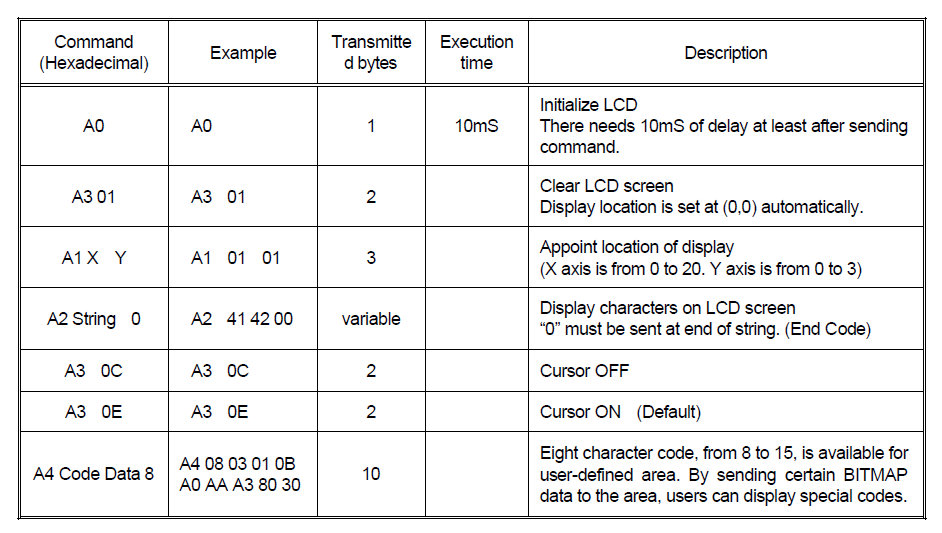
\includegraphics[width=14cm,height=8cm]{images/commandesLCD.png}
				\paragraph{\textit{Figure 0.2.2 : Tableau des différentes commandes du LCD, ELCD Datasheet}}
				\paragraph{}
					\emph{LCD\_ecrire} permet d'envoyer des chaînes de caractères dans le THR, bit par bit.
					\emph{LCD\_clear} envoie la commande de reset de l'écran du LCD.
					\emph{LCD\_init} permet d'initialiser le LCD. Il faut attendre 10ms après l'envoi de cette commande pour que le LCD soit fonctionnel. Cette attente est générée dans la fonction main du projet, car le fichier lcd.c est appelé régulièrement, toutes les secondes. C'est pourquoi \emph{LCD\_init} est appelée directement dans le main.
					\emph{LCD\_positionCurseur} permet de placer le curseur à l'endroit voulu sur l'écran.

				\paragraph{}
					Ces fonctions sont les fonctions de base pour pouvoir afficher quelque chose sur le lCD. Intuitivement, avant d'utiliser le Time-guard pour générer une pause entre chaque envoi de caractère, j'avais créé une fonction \emph{LCD\_break} qui s'appuyait sur les break générés par l'USART. Cependant, ceci ne résolvait rien : le break s'appuyait sur le THR, il mettait des données compréhensibles par l'USART et enlevait le bit US\_TXRDY, et pour ensuite sortir du break enlevait le bit US\_TXEMPTY dans le US0\_CSR, puisqu'au final, après l'envoi de ces commandes, l'attente n'était toujours pas gérée. Cela accentuait mes problèmes.

			\subsection{Etat final}
				Le LCD est opérationnel. Toutes les fonctions marchent correctement. Pour pousser le travail plus loin, j'ai voulu créer la fonction de bienvenue, avec une petite animation où le message de bienvenue se déplacerait sur l'écran. Il fallait donc créer une fonction qui permettrait d'effacer les caractères un à un à la position voulue. La fonction \emph{LCD\_positionCurseur} étant opérationnel, je n'avais plus qu'à m'occuper du "clear local", qui se basait sur le remplacement d'un caractère par un espace. Néanmoins, cette fonction ne fonctionne pas correctement. Le bout du travail aurait été de créer des caractères nous-mêmes, et ensuite, via ce travail, créer des animations plus poussées, qui se jouerait au pixel près. Peut-être que cela sortirait du cadre du projet.


\part{Le son\\-\\Fabien \bsc{Jaraczewski}}
\section{Introduction}
Le but de cette partie est d'implémenter 3 fonctions utilisables dans le main :

\begin{itemize}
\item \texttt{SON\_jouerBipOk} : génère un bip correspondant à une commande reçue correcte
\item \texttt{SON\_jouerBipKo} : génère deux bips, correspondant à une commande reçue non autorisée ou incorrecte
\item \texttt{SON\_jouerAlarme} : génère un son de 5 secondes en continu, pour un seuil d’alarme atteint tant qu’on n'appuie pas sur une touche précise de la télécommande
\end{itemize}

Par la suite, la fonction alarme est devenue une série de bips durant 6 s, et une autre fonction a été créée, utilisant plusieurs notes différentes, pour jouer une musique au démarrage de la carte.

Je me suis focalisé sur la mise en oeuvre des fonctions ci-dessus par le biais d'un créneau envoyé directement sur la sortie.
J'utilise le timer TC4 du processeur ARM, et le signal est généré sur le port A, relié à la broche n$^\circ$4.

\section{Initialisations}
Les différentes fonctions d'initialisations sont regroupées dans la fonction \texttt{SON\_initialisation} exécutée dans le main, ainsi que la fonction \texttt{SON\_start\_timer4} qui démarre le timer.
L'initialisation du timer inclus son alimentation, le mode choisi (\emph{waveform}), la division de l'horloge de base du timer, l'autorisation des interruptions, ainsi que la définition des rôles des registres RA et RC utilisés pour générer le créneau.
J'ai choisi de prédiviser la fréquence de l'horloge de base du timer (32 MHz) par 1024 afin d'avoir des fronts montants et donc des comparaisons le moins souvent possible, ce qui permet de ne pas utiliser pour rien le processeur tout en pouvant générer les fréquences voulues.

L'initialisation du timer inclus son alimentation, le mode choisi (waveform), la division de l'horloge de base du timer, l'autorisation des interruptions, ainsi que la définition des rôles des registres RA et RC utilisés pour générer le créneau.
J'ai choisi de prédiviser la fréquence de l'horloge de base du timer (32 MHz) par 1024 afin d'avoir des fronts montants et donc des comparaisons le moins souvent possible, ce qui permet de ne pas utiliser pour rien le processeur tout en pouvant générer les fréquences voulues.

\begin{verbatim}
// alimentation du timer 4
APMC_PCER = APMC_PCER | (1<<TC4_ID);
// prédivision de l'horloge par 1024
TC_CLKS_MCK1024 |
// T est la période du créneau correspondant à un LA 440
TC4_RC = T;
TC4_RA = 2*T;
\end{verbatim}

Le registre RA est initialisé à une valeur supérieure à RC pour ne pas former de créneau ;
on lui attribuera les différentes valeurs correspondant aux fréquences des notes, ainsi qu'à RC, en fonction de la note, donc de la période du créneau, voulue.
L'initialisation du contrôleur d'entrées-sorties contient l'alimentation et le choix de la broche affectée.

\texttt{PIOA\_PDR = P4; // sortie TIOA branchée sur la broche n$^\circ$4}

L'initialisation du convertisseur numérique –> analogique (pas encore utilisé) contient l'alimentation, un temps d'attente (>5$\mu$s) pour que le CNA démarre, la sélection du port A pour tranférer les données sur 10 bits.
J'avais prévu initialement d'utiliser le CNA pour transmettre un signal quasi-sinusoïdal généré par un tableau d'échantillonnage, mais par manque de résultats probants, j'ai préféré jouer les différentes notes de musique à l'aide de créneaux aux périodes correspondantes, puisque les tests sur la carte ont montré que le résultat était concluant.

Le code d'initialisation du CNA ci-après n'est donc pas utilisé :

\begin{verbatim}
/** initialisation du convertisseur numérique -> analogique */
void SON_init_DAC(void)
{
int cpt = 0;
APMC_PCER = APMC_PCER | (1<<DAC0_ID); // alimentation du convertisseur numérique
-> analogique
while (cpt < 20)
// boucle d'attente dûe au temps de startup
{ cpt++; }
DAC0_CR = DAC_SWRST; // réinitialisation
DAC0_MR = DAC_TTRGEN_EN | // transfert synchronisé par le timer trigger
DAC_TRG_TIOA4 | DAC_10_BIT_RES; // sélection de TIOA pour actualiser les données,
envoyées sur 10 bits
DAC0_DHR = DAC_DATA_10BITS;
// transfert des données sur 10 bits vers le registre
tampon
DAC1_IDR = DAC_DATRDY;
// désactivation des interruptions
}
\end{verbatim}

L'initialisation du contrôleur d'interruptions inclus son alimentation, la définition de son ordre de priorité, l'appel de la fonction d'interruption \texttt{SON\_interrupt}, l'activation des interruptions.

\section{Fonctions}
La fonction \texttt{SON\_jouerBipOk} génèrera un bip de 200ms (un LA 440).
Pour ce faire, on attribue à RA une valeur plus grande que RC pour ne pas générer de créneau après le temps voulu.

\begin{verbatim}
flagBip = 1; // drapeau mis à 1 pour rentrer dans la boucle de l'interruption
TC4_RA = T/2; // ré-initialisation du registre RA pour former un créneau
while (compteurSon < F*dureeBip);
// arrêt du bip quand la durée est égale à 200ms
TC4_RA = 2*T;
// RA est mis à une valeur supérieure à RC pour empêcher le créneau
\end{verbatim}

\begin{center}
	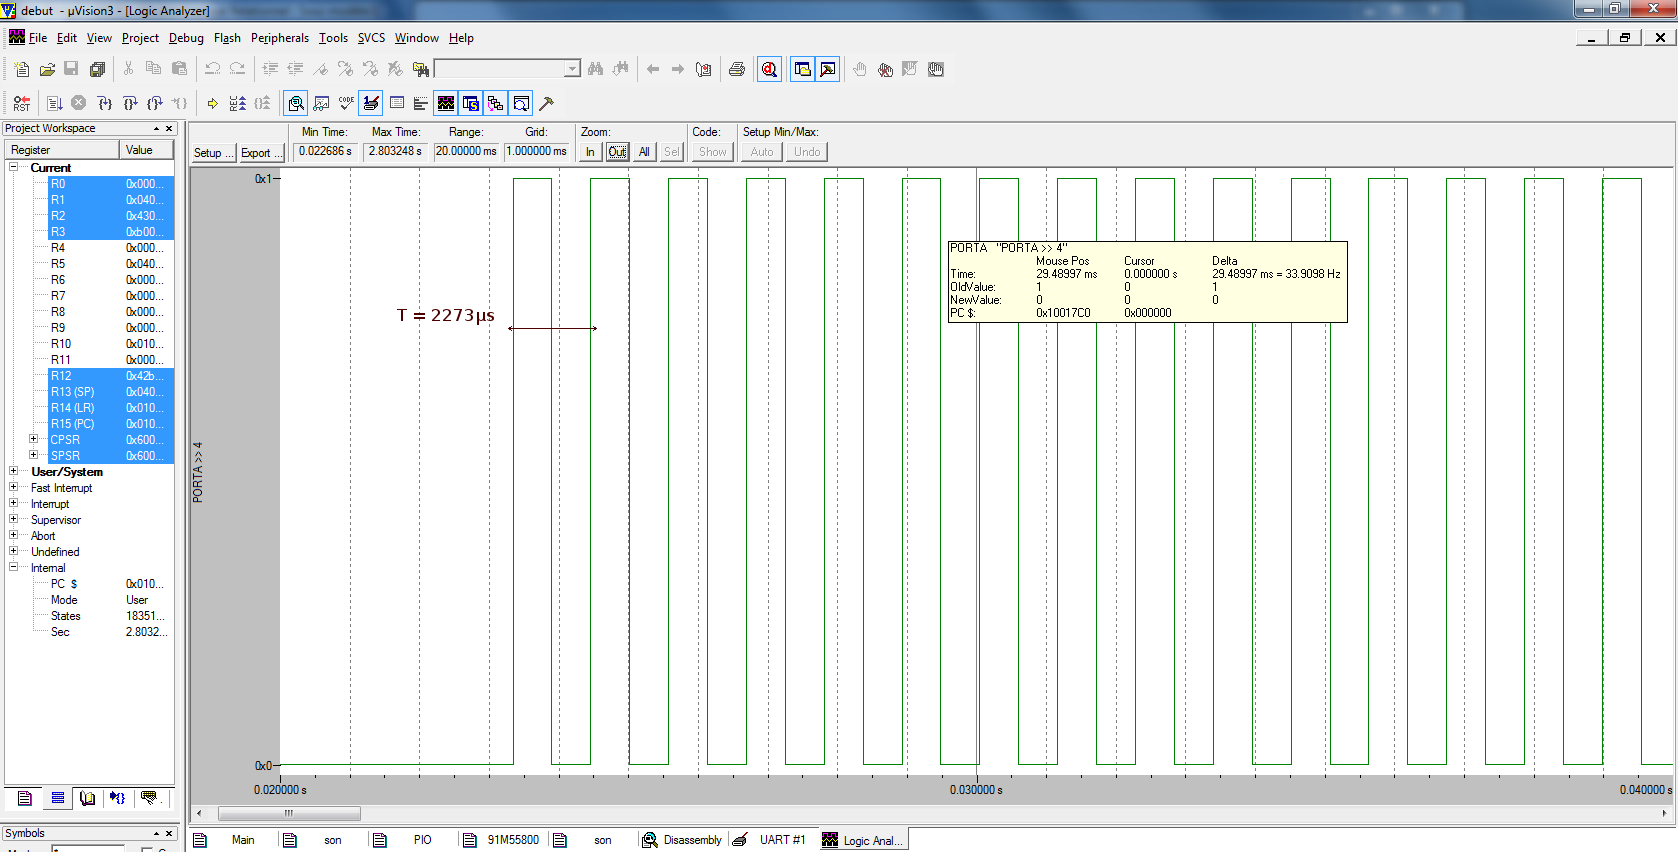
\includegraphics[scale=0.2]{images/SON_fig1.png}
\end{center}

La fonction \texttt{SON\_jouerBipKo} génèrera un bip de 200ms, puis un silence de 100ms, puis un nouveau bip de 200ms.
Au bout de 300ms, on remet RA à sa valeur initiale (moitié de RC) pour générer à nouveau un créneau, puis on empêche le créneau de se créer de la même façon après 500ms.

\begin{verbatim}
while(compteurSon < 1.5*F*dureeBip);
// deuxième bip après une pause de durée moitié d'un bip
TC4_RA = T/2;
// ré-initialisation du registre RA pour former un créneau
while(compteurSon < 2.5*F*dureeBip);
// arrêt du deuxième bip
TC4_RA = 2*T; // RA est mis à une valeur supérieure à RC pour empêcher le créneau
compteurSon = 0; // remise à zéro du compteur une fois les 2 bips effectués
\end{verbatim}

La fonction \texttt{SON\_jouerAlarme} génère des bips rapprochés pendant 6 secondes, ce qui correspond à 12 appels à la fonction \texttt{SON\_jouerBipKo}, contrôlés par l'incrémentation d'un compteur local.
La fonction \texttt{SON\_jouerPrintemps1} est basée sur le même principe que \texttt{SON\_jouerBipKo}, mais à chaque fois on change la période du créneau pour obtenir la note voulue.
Les périodes des 8 notes sont définies dans le fichier son.h, en tenant compte de la prédivision de l'horloge par 1024.
Ainsi, la période de la note LA par exemple, est obtenue par le calcul suivant :

\[
{32 \over 1024} \times {1 \over 440} = 7,10227.10\up{-5} s
\]

De même pour la fonction \texttt{SON\_jouerPrintemps2}.

\begin{verbatim}
TC4_RC = t_do;
TC4_RA = t_do/2;
dureeBip = 0.2;
// bip de 200ms
while(compteurSon < Do*dureeBip);
// arrêt de la note DO quand la durée est égale à 200ms
TC4_RA = 2*T;
// RA est mis à une valeur supérieure à RC pour empêcher le créneau
while(compteurSon < 1.5*Do*dureeBip);
// deuxième note après une pause de durée moitié d'un bip
TC4_RC = t_re;
TC4_RA = t_re/2;
// ré-initialisation des registre RA et RC pour former un créneau
correspondant à la note RÉ
while(compteurSon < 2.5*Re*dureeBip);
// arrêt de la deuxième note
\end{verbatim}

\section{Simulations}
À l'aide du logiciel $\mu$Vision3, j'ai réalisé des simulations de génération du signal créneau ;
le test suivant appelle toutes les fonctions utilisées, en introduisant un temps d'attente entre chaque :

\begin{verbatim}
int main(void)
{
int cpt = 0;
AIC_IDCR=0xFFFFFFFF;
AIC_ICCR=0xFFFFFFFF;
SON_initialisation();
SON_jouerPrintemps1();
//Désactive toutes les interruptions
SON_jouerPrintemps2();
while (cpt < 500000)
{cpt++;}
SON_jouerBipOk();
while (cpt < 1000000)
{cpt++;}
SON_jouerBipKo();
while (cpt < 1500000)
{cpt++;}
SON_jouerAlarme();
while (1);
}
\end{verbatim}

\begin{center}
	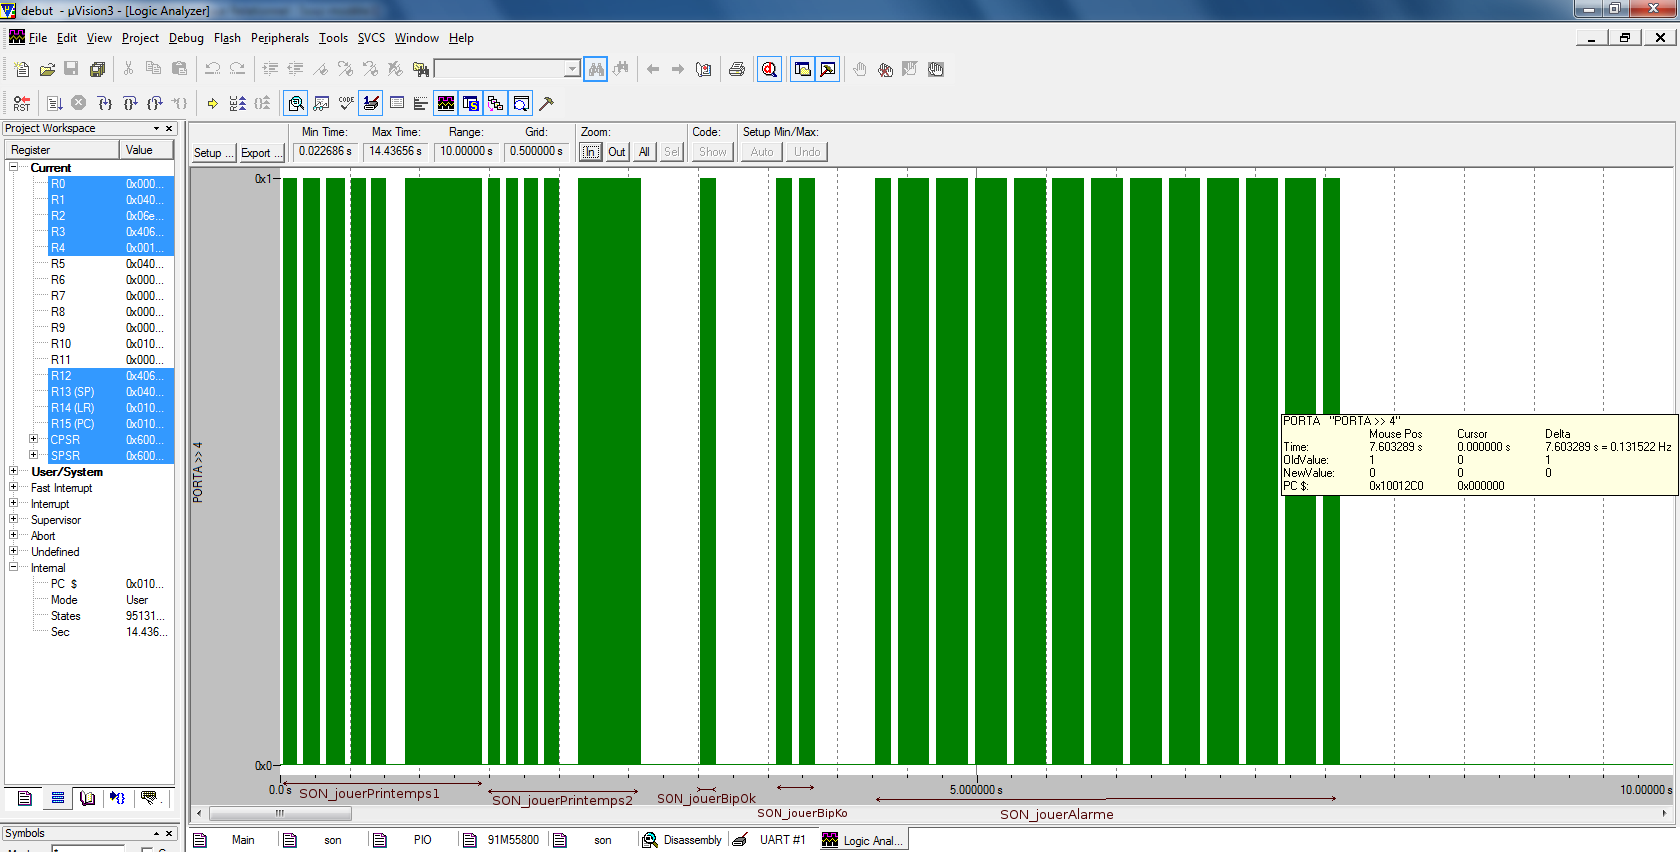
\includegraphics[scale=0.2]{images/SON_fig2.png}
\end{center}

\section{Apport personnel}
Je voulais au départ commencer par faire les fonctions du son en générant un créneau et ensuite les transcrire en utilisant le convertisseur numérique/analogique pour générer des notes, mais j'ai finalement abandonné la deuxième solution et ai conservé l'outil créneau.
Les problèmes rencontrés ont été une difficulté à appréhender la documentation du micro-contrôleur, et des problèmes logiciels dûs à $\mu$Vision.
Pour générer le créneau, je me suis inspiré du code réalisé auparavant en TP sur le robot.
Une fois le créneau fonctionnel (après tests en simulation et sur la carte), j'ai rencontré des difficultés à gérer l'arrêt et la reprise des bips, on a donc mis sur cette tâche Hugo Vérité et Kévin Vytheligum, qui m'ont aidé sur cette partie.

Ce projet m'a permis de mieux comprendre comment fonctionne un micro-contrôleur ARM, et m'a également apporté une expérience du travail en équipe (répartition des tâches, gestion des emplois du temps...).


\chapter*{Conclusion}
Le projet de la station météo s’est révélé très enrichissant pour chacun des membres de l’équipe.
Chacun était en charge d’un composant essentiel de la station, et cela a permis d’appréhender pleinement les responsabilités et les difficultés qu’apporte le travail en équipe.
Les difficultés rencontrées ont été réellement formatrices.

La station est presque au point.
Outre la télécommande et la température, le reste de la station est fonctionnel.
Il ne reste qu’à améliorer l’interface de l’utilisateur pour que la station soit plus facile et agréable à prendre en main.
Le travail qu’il reste à fournir est donc de l’ordre de l’optimisation.

L’équipe tient à remercier le personnel encadrant, à savoir Messieurs EL FALOU et COURTAY pour leur contribution qui devait certes rester minime, mais décisive à chaque intervention.

\end{document}
